\documentclass{article}
\usepackage{hyperref}
\usepackage{fancyhdr}
\usepackage{tikz}
\usepackage{multicol}
\usepackage{pgf}
\usepackage{graphicx} 
\usepackage{array}
\usepackage{mdframed}
\usepackage[left=1in,right=1in,top=1in, bottom=1in]{geometry}
\usepackage{float}
\usepackage{color}
\usepackage{xcolor}
\usepackage[utf8]{inputenc}
\usepackage[arabic]{babel}
\usepackage{polyglossia}
\usepackage{fontspec}
\setmainlanguage{arabic}
\newfontfamily\arabicfont[Script=Arabic]{Tajawal}
\usepackage{tocloft}
\addtolength{\cftsecnumwidth}{12pt}
\addtolength{\cftsubsecnumwidth}{12pt}
\setlength{\cftsubsecindent}{30pt}
\usepackage{endnotes}
\usepackage{scrextend}
\usepackage[utf8]{inputenc}
\usepackage{url}
\usepackage{paralist}
\newcolumntype{R}[1]{>{\let\newline\\\arraybackslash\hspace{0pt}}m{#1}}

\usepackage{authblk}
\usepackage{tablefootnote}
\usepackage{todonotes}
\usepackage{lscape}
\usepackage{chronology}
\usepackage{enumitem, amssymb}
\usepackage{booktabs} 
\usepackage{dcolumn}
\definecolor{abblue}{RGB}{30,150,186}
\definecolor{abblueD}{RGB}{44,143,159}
\definecolor{aborange}{RGB}{223,109,33}

\pagestyle{fancy}
\fancyhf{}
\renewcommand\headrule{}
\fancyhead[L]{\color{gray}\footnotesize{الباروميتر العربي} \\
	\color{gray}\footnotesize{تقرير الجزائر}}
\cfoot{\color{gray}\footnotesize{الباروميتر العربي}}
\rfoot{\color{gray}\footnotesize{ \thepage}}
\usepackage{background}
\hypersetup{colorlinks=false,pdfborder=0 0 0,citebordercolor={0 0 0}}


\begin{document}
	\newpage
	\backgroundsetup{
		scale=1,
		color=black,
		opacity=1,
		angle=0,
		contents={%
			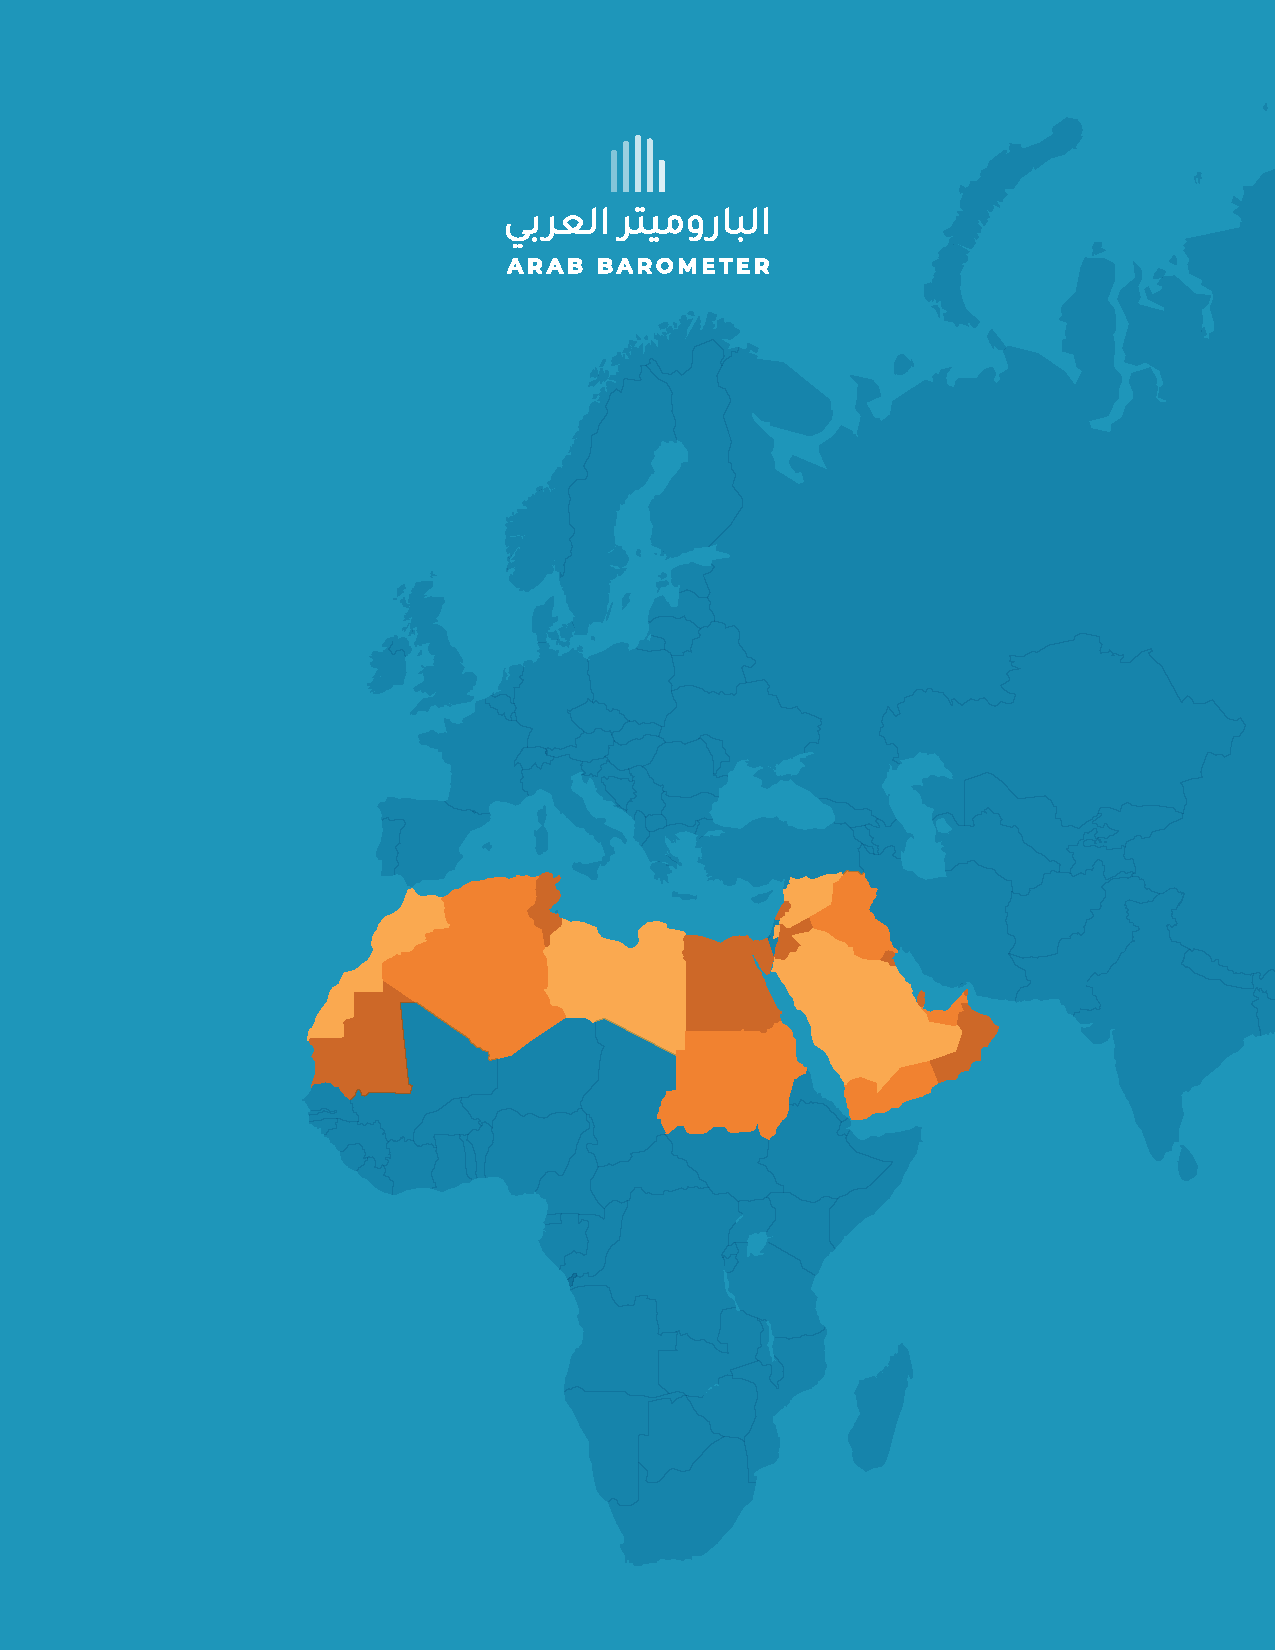
\includegraphics[width=\paperwidth,height=\paperheight]{AB_FrontCover.pdf}
		}%
	}
	\newgeometry{left=1in,right=1in,top=1in, bottom=1in}
	\pagestyle{empty} 
	\vspace*{2in}
	\begin{center}
		\color{white}\Large\textbf{تقرير الجزائر} \\
		\vspace*{0.5in}
		\color{white}\large{٢٠١٩} \\
		\vspace*{4in}
		\color{white}\large{الباروميتر العربي، الدورة الخامسة} \\
	\end{center}
	%%%%%%%%%%%%%%%%%%%%%%%%%%%%
	\newpage\backgroundsetup{contents={}}
	\color{gray}
	%%%%%%%%%%%%%%%%%%%%%%%%%%%%
	\color{gray}
	\pagestyle{fancy}
%%%%%%%%%%%%%%%%%%%%%%%%%%%%
	\pagebreak
	\section*{الملخص التنفيذي}
	
 بدءاً من فبراير/شباط 2019، بدأ الكثير من المواطنين في التظاهر، ما أدى في النهاية إلى استقالة الرئيس عبد العزيز بوتفليقة. عشية الاحتجاجات، لم يكن المواطنون الجزائريون يشعرون فقط بالإحباط العميق جراء الظروف الاقتصادية، إنما كانوا يشعرون بالإحباط من النظام بأكمله. فمدركات حالة الاقتصاد ومقدار التفاؤل إزاء مستقبل البلاد شهدت انحداراً كبيراً منذ 2013، لكن أقل من النصف قالوا إن الاقتصاد هو مشكلة الجزائر الرئيسية. إذ قالت نسبة تكاد تكون مماثلة إن الفساد أو جودة الخدمات العامة هي التحدي الأكبر الذي يواجه البلاد. 
	
 يشعر الجزائريون بمقدار محدود من الثقة بحكومتهم فيما يخص اضطلاعها بواجباتها. يقول شخص واحد من كل 10 أشخاص فقط إن الحكومة تحسن التعامل مع ملفات البطالة أو التضخم أو خفض أوجه اللامساواة. وبالرغم من السلم الأهلي الذي ساد إبان الحرب الأهلية في التسعينيات، فلحظة انطلاق المظاهرات كان النصف فقط يرون أن الحكومة تحسن توفير الأمن، ما يوحي بتفشي الإحباط من حُكام الجزائر. وفي مواجهة هذه التحديات العريضة، يسعى ثلث الجزائريين تقريباً لمغادرة بلدهم سعياً وراء حياة أفضل بالخارج.
	
	
 ويعد تأييد الديمقراطية منخفض نسبياً في الجزائر مقارنة بدول أخرى في الشرق الأوسط وشمال أفريقيا. لدى طرح سؤال عما إذا كانت الديمقراطية هي النظام الأفضل دائماً، أجاب أقل من النصف بتأييد المقولة المذكورة، في حين قال الثلث تقريباً إن الحكومة غير الديمقراطية قد تكون أفضل أحياناً، وقال 1 من كل 5 أشخاص إن شكل الحكومة لا يهم. وفي الوقت نفسه يقول عدد قليل من الجزائريين إن بلدهم حالياً ديمقراطي، رغم أن شخص من كل 10 أشخاص يعرّف الديمقراطية بصفتها تتمثل في الانتخابات الحرة والنزيهة.
	
 دارت الحرب الأهلية الجزائرية في تسعينيات القرن العشرين بين القوى الإسلامية وخصومها الأكثر علمانية. وخلال العقدين التاليين على النزاع، ظلّ هذا الانقسام ظاهراً بقوة. هناك نسب متساوية تقريباً من الجزائريين تدعم وتعارض زيادة دور الدين في الحياة العامة.
	
 وفي الوقت نفسه، فعلى الرغم من أن الجزائريين يتزايد إقبالهم على القول بأن بلدهم يجب أن ينفتح على العالم الخارجي، فهناك قلة – نسبية – ترغب في تقوية العلاقات بالقوى العالمية أو الإقليمية الرئيسية. بالمثل، فهناك قلة ترغب في زيادة المساعدات الواردة من العالم الخارجي، ما يعكس ارتياب عميق نحو دوافع تقديم المساعدات. الغالبية تقول إن الدافع الرئيسي لدى الدول الأجنبية التي تقدم المساعدات هو كسب النفوذ على الجزائر.
	
 هذه هي بعض النتائج الأساسية لاستطلاع الرأي الممثل للرأي العام على مستوى الجزائر الذي أجراه الباروميتر العربي   في الفترة من 30 يناير/كانون الثاني إلى 18 فبراير/شباط 2019. شهد الاستطلاع إجراء 2332 مقابلة وجهاً لوجه بأماكن سكن المبحوثين، وله هامش خطأ بلغ ±2 بالمئة، وبلغت نسبة تعاون المبحوثين 76.7 بالمئة.
	\pagebreak
%%%%%%%%%%%%%%%%%%%%%%%%%%%%%%
%%%%% 

\section*{الحالة الاقتصادية}

 في عام 2019 خرج الجزائريون إلى الشوارع في مظاهرات حاشدة، ليس فقط احتجاجاً على الرئيس السابق عبد العزيز بوتفليقة، إنما أيضاً ضد النظام الحاكم للبلاد. في واقع الأمر، تُظهر نتائج الاستطلاع أن حالة السخط في الجزائر لم يحركها سبب وحيد، إنما جملة من المظالم. لدى طرح السؤال حول التحدي الأهم الذي يواجه البلاد، أجاب 4 من كل 10 أشخاص بأن المشكلات الاقتصادية هي الأكثر إلحاحاً. وفي الوقت نفسه يقول شخص من كل 5 أشخاص (22 بالمئة) إنه الفساد أو الخدمات العامة (19 بالمئة) في حين يقول آخرون إنه الأمن الداخلي (5 بالمئة) أو عوامل أخرى. 
	
	\begin{center}
	\begin{figure}[H]
		\centering
		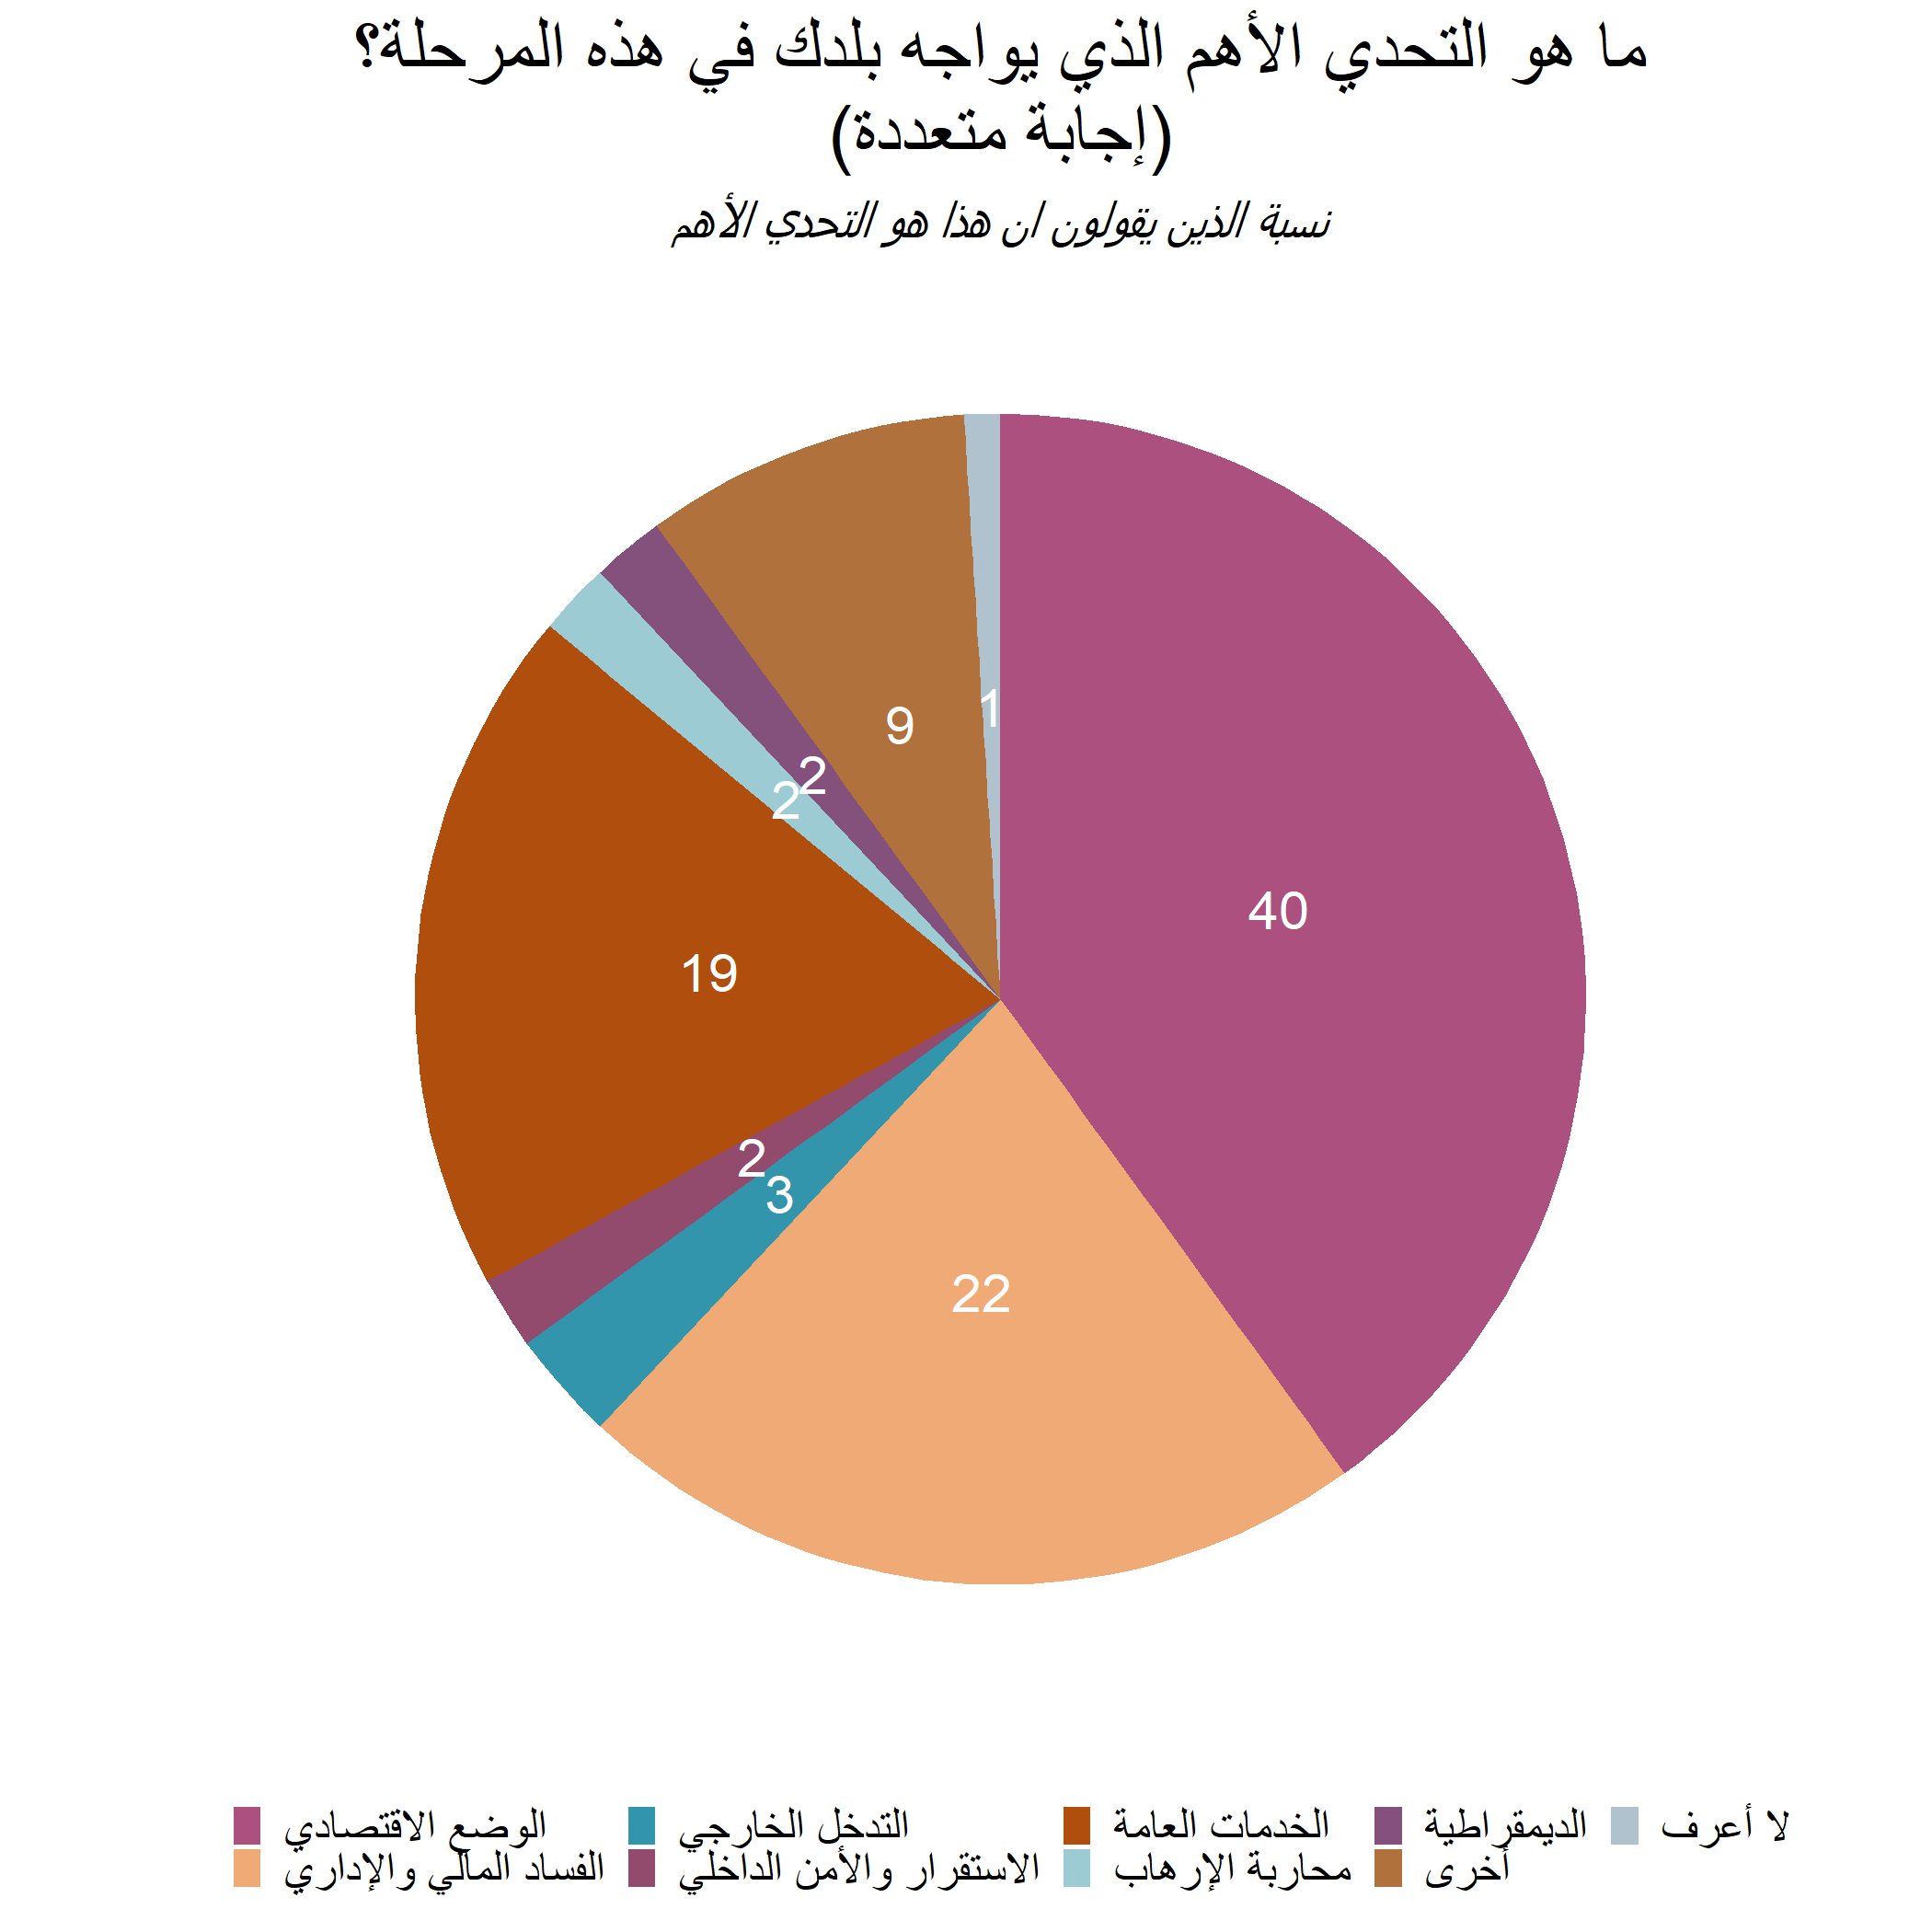
\includegraphics[width=13cm]{Q206.png}
	\end{figure}
	\end{center}

 يعتبر 13 بالمئة فحسب من الجزائريين أن الاقتصاد جيد، وهي النسبة التي شهدت انحداراً كبيراً للغاية منذ 2013 (53- نقطة). بعد الانتفاضات العربية، زادت الحكومة الجزائرية من برامج الدعم الاقتصادي للمواطنين ونفذت سياسات اقتصادية أخرى كانت مفيدة للمواطنين العاديين، والفضل في هذا – جزئياً – يعود إلى ارتفاع أسعار النفط. لكن مع انهيار أسعار النفط عالمياً في 2014، واجهت الجزائر – وهي الدولة الوحيدة في الشرق الأوسط وشمال أفريقيا العضوة بالأوبك من خارج دول مجلس التعاون الخليجي – تحديات اقتصادية وتدهور المقدرات الاقتصادية للمواطنين.
	
	\pagebreak
	\begin{center}
	\begin{figure}[H]
		\centering
		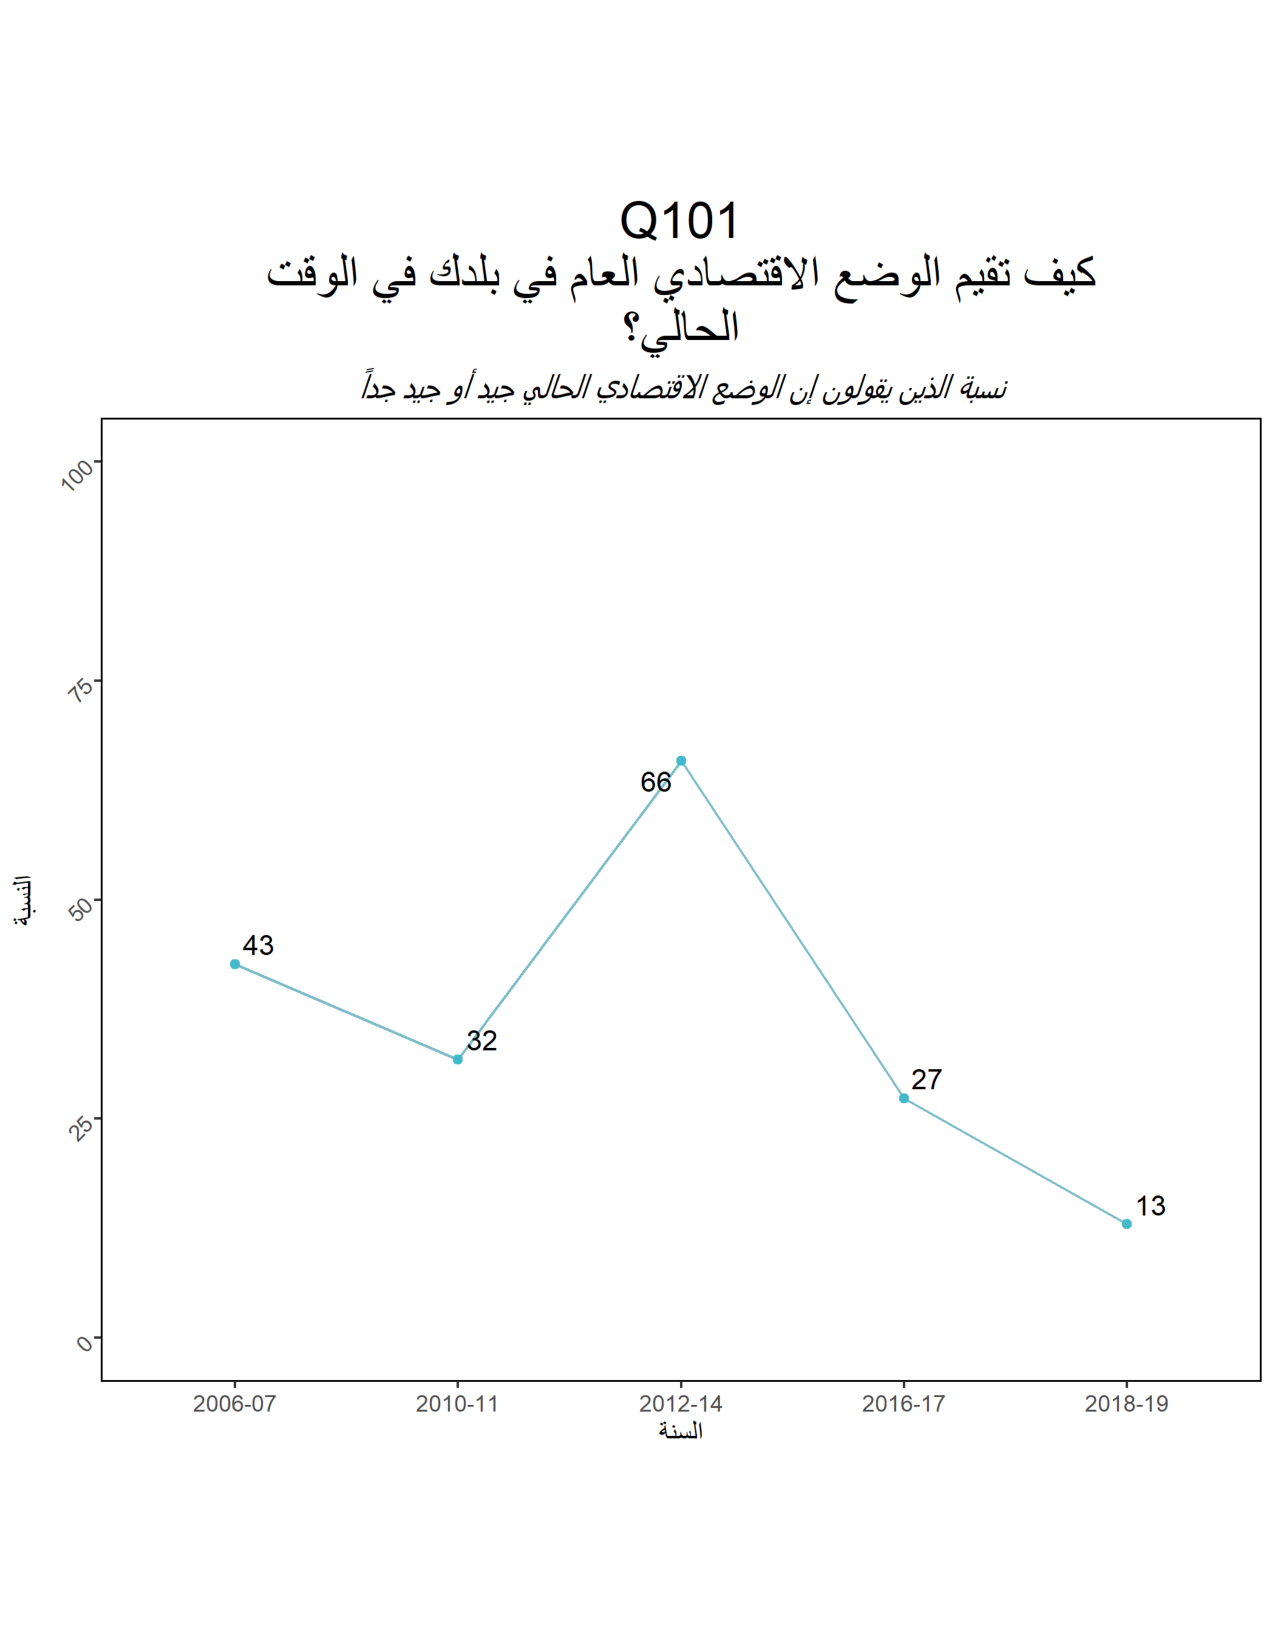
\includegraphics[width=13cm]{Q101_.png}
	\end{figure}
	\end{center}

 أيضاً، انحدرت نسبة التفاؤل الاقتصادي كثيراً على مدار السنوات الأخيرة، بعد أن بلغت ذروتها في 2013 بواقع 63 بالمئة، ثم انحسرت 41 نقطة مئوية لتبلغ 22 بالمئة في 2019. يجدر بالملاحظة أن التفاؤل الاقتصادي متماثل في النسب بين الشباب والكبار، والذكور والإناث، والأثرياء والفقراء، وسكان الحضر والريف، والأعلى تعليماً والأقل تعليماً. لكن هناك اختلافات جغرافية مهمة: فالثلث (34 بالمئة) ممن يعيشون بالمنطقة الوسطى المحيطة بالجزائر العاصمة يتوقعون أن يتحسن الاقتصاد، مقارنة بـ 23 بالمئة ممن يعيشون بمناطق الشمال الغربي و13 بالمئة من سكان الشمال الشرقي.
	
%	\pagebreak
	\begin{center}
		\begin{figure}[H]
			\centering
			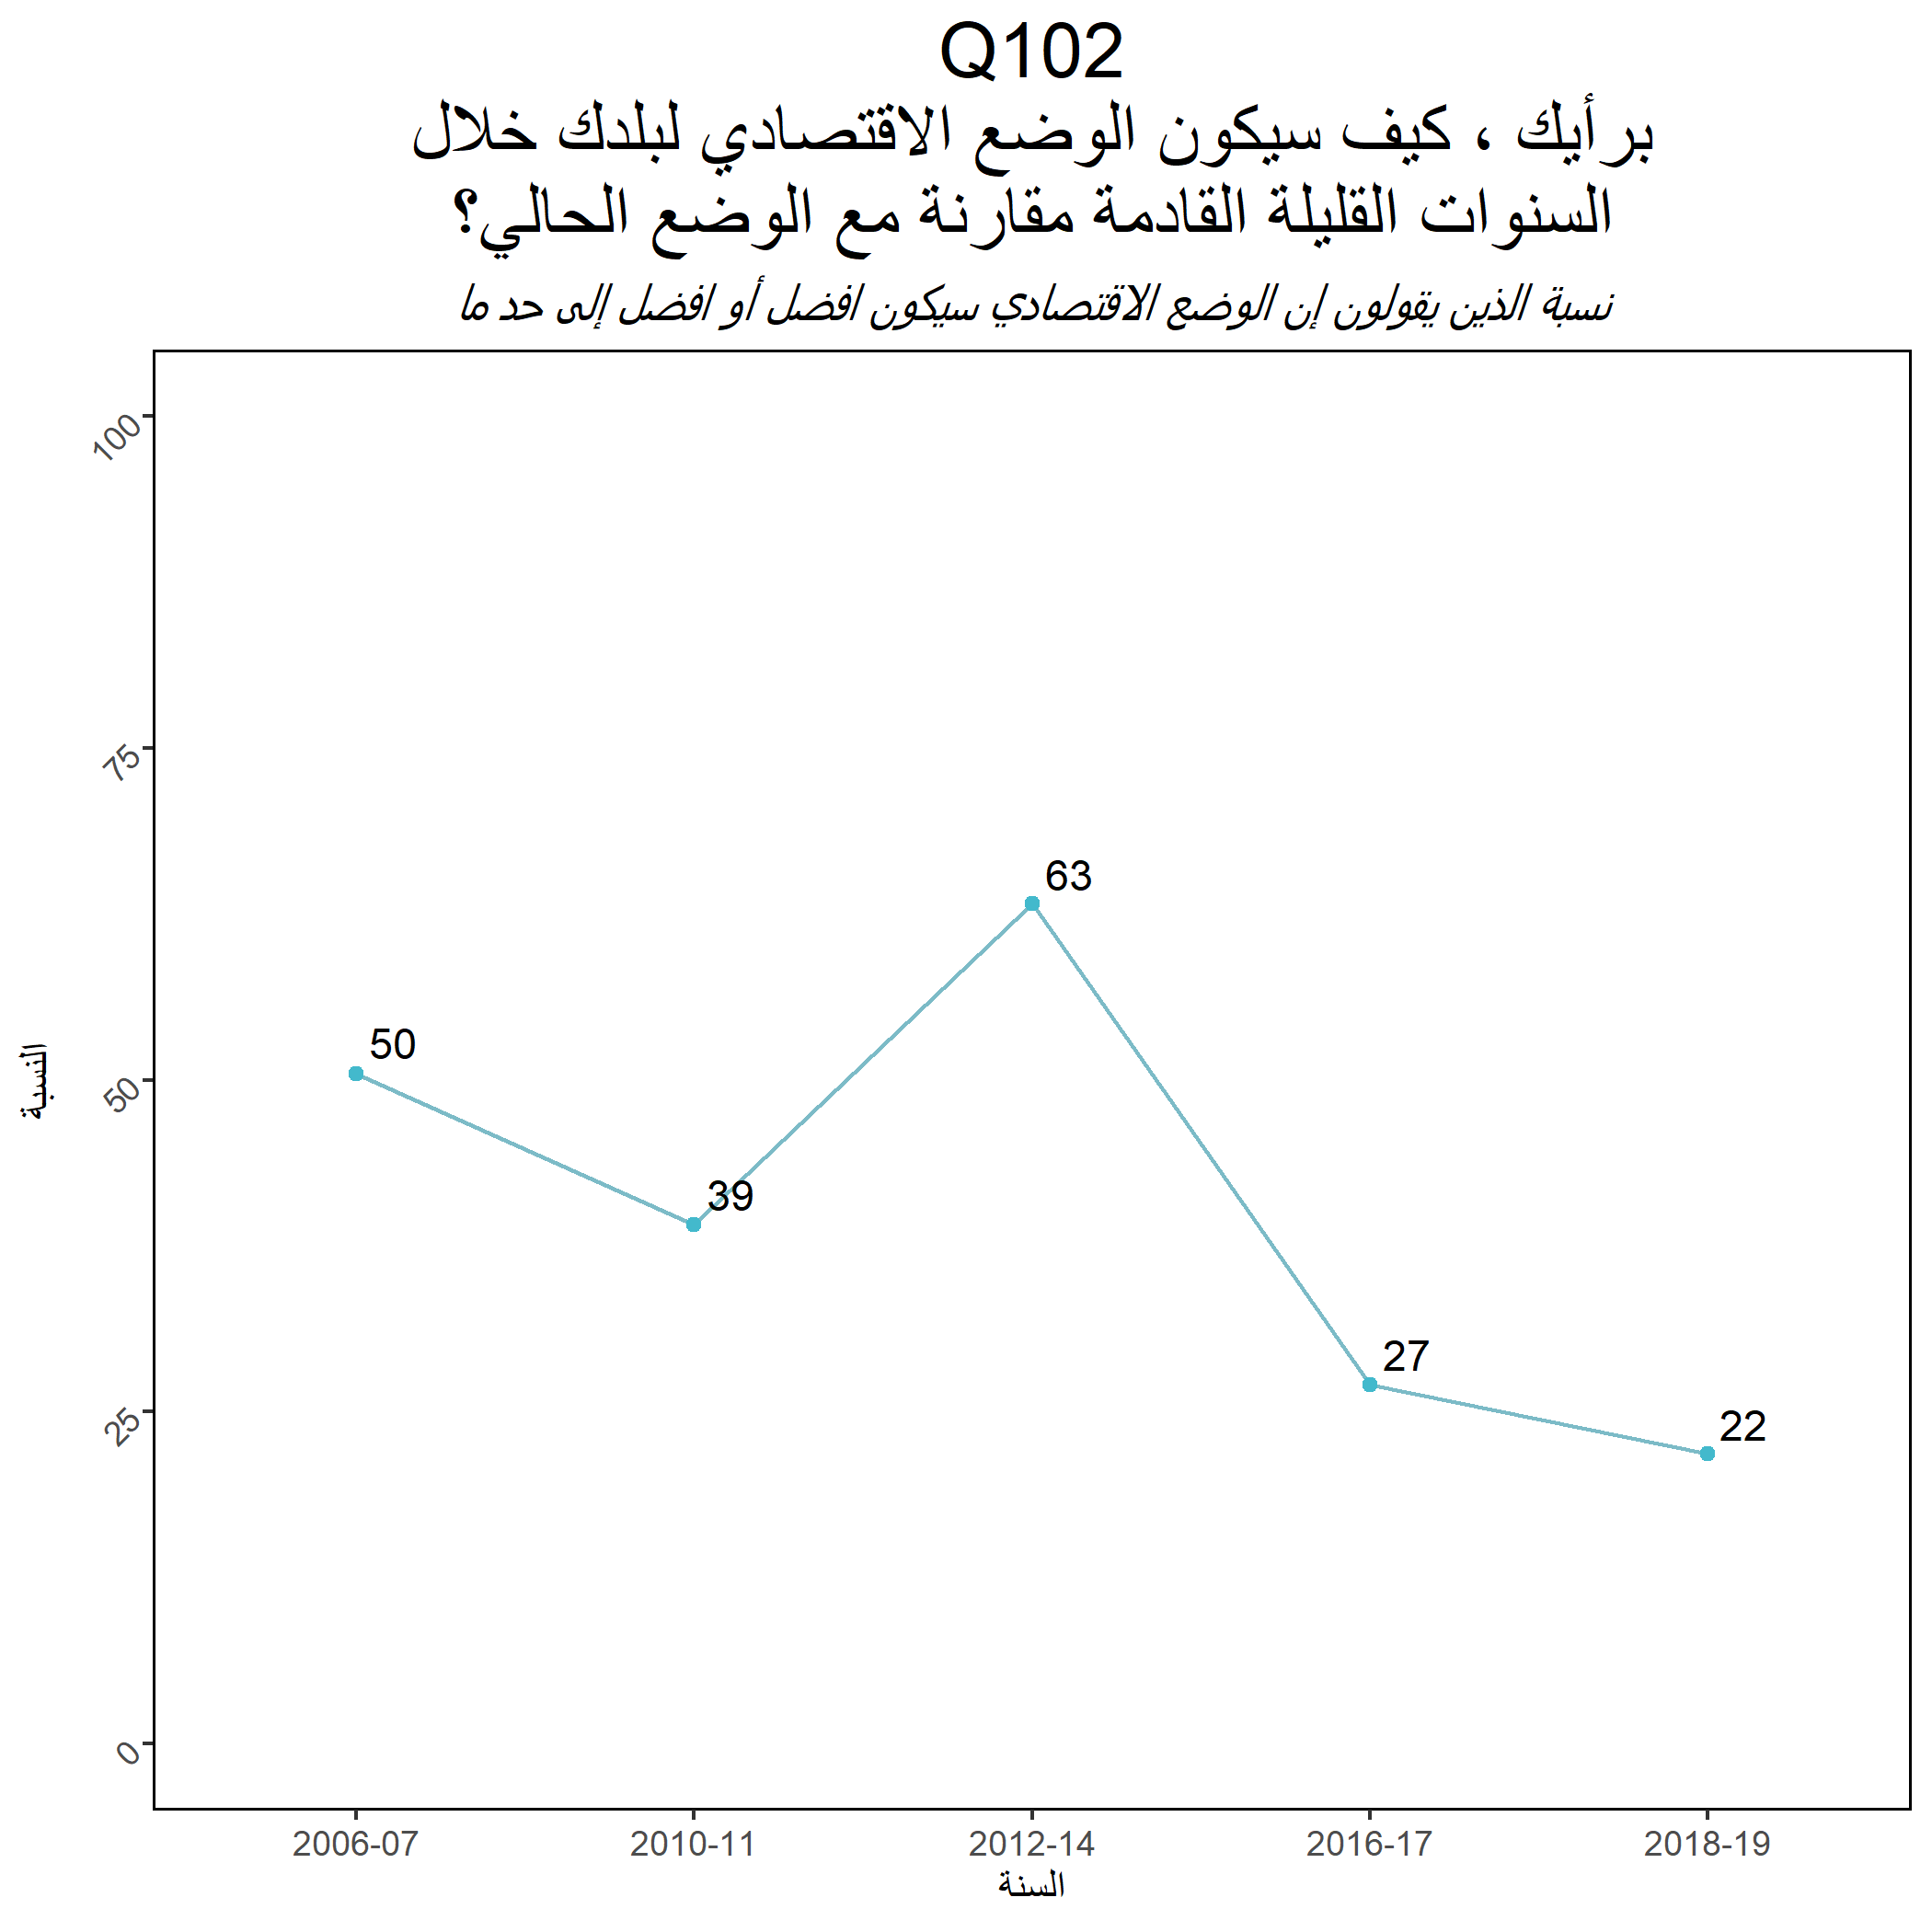
\includegraphics[width=13cm]{Q102_.png}
		\end{figure}
	\end{center}
	
\section*{الهجرة}

 يفكر 3 من كل 10 جزائريين في الهجرة، وهي النسبة التي زادت 8 نقاط مئوية منذ 2016. يمثل هذا التغير انعكاساً في التوجه السابق الخاص بتراجع نسبة الراغبين في الهجرة، هو قائم منذ فترة طويلة، في الفترة من 2006 إلى 2016، ما يُظهر حدوث تغير هام في الاتجاهات.
	
%	\pagebreak
	\begin{center}
		\begin{figure}[H]
			\centering
			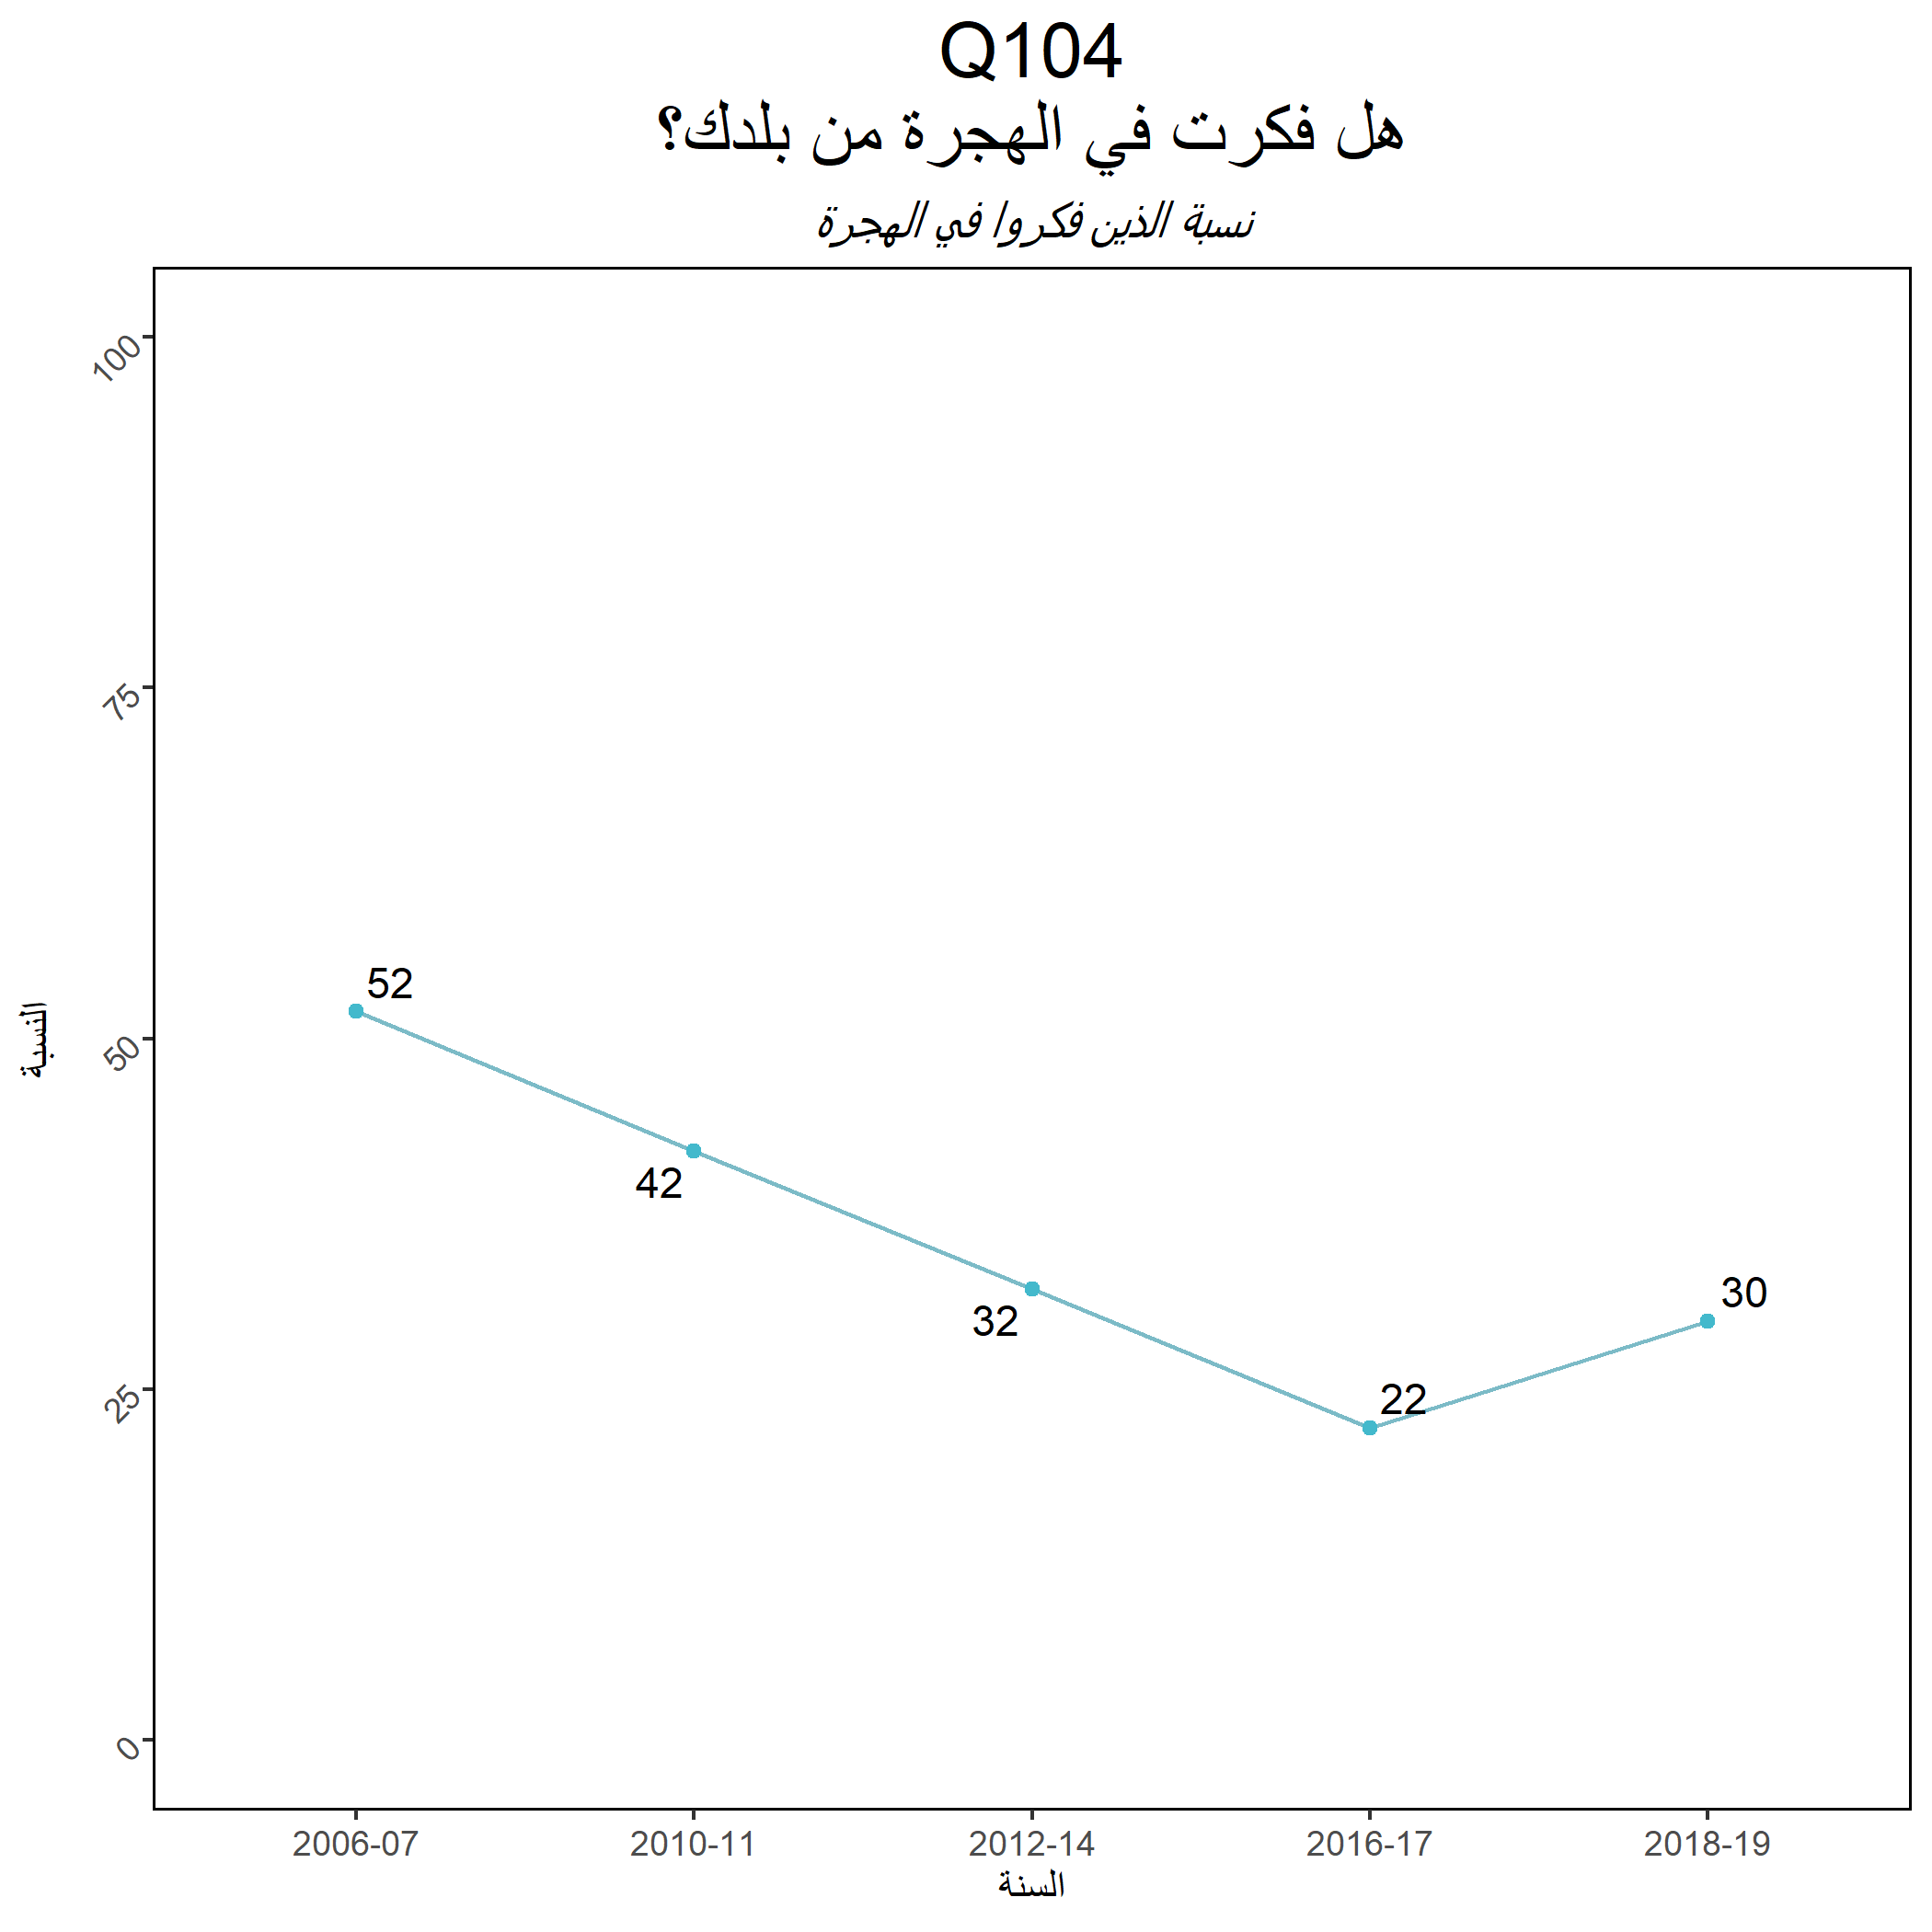
\includegraphics[width=13cm]{Q104_.png}
		\end{figure}
	\end{center}
	
%	\pagebreak	
 الجزائريون الأصغر سناً هم الأكثر إقبالاً بكثير على التفكير في الهجرة مقارنة بالأجيال الأكبر. ويجدر بالملاحظة أن أكثر من نصف (56 بالمئة) أفراد الشريحة العمرية 18 إلى 29 عاماً يفكرون في مغادرة البلاد، مقارنة بـ 35 بالمئة في الشريحة العمرية 30 إلى 39، و17 بالمئة في الشريحة العمرية 40 إلى 49، و10 بالمئة ممن تبلغ أعمارهم 50 عاماً فأكبر. كما تخاطر الجزائر بفقدان أفضل وألمع عناصرها البشرية، إذ أن نحو نصف (46 بالمئة) حملة الشهادات الجامعية يفكرون في الهجرة، مقارنة بشخص واحد من كل 5 أشخاص (19 بالمئة) من أصحاب التعليم الأساسي.

    

			\begin{figure}[H]
				\centering
				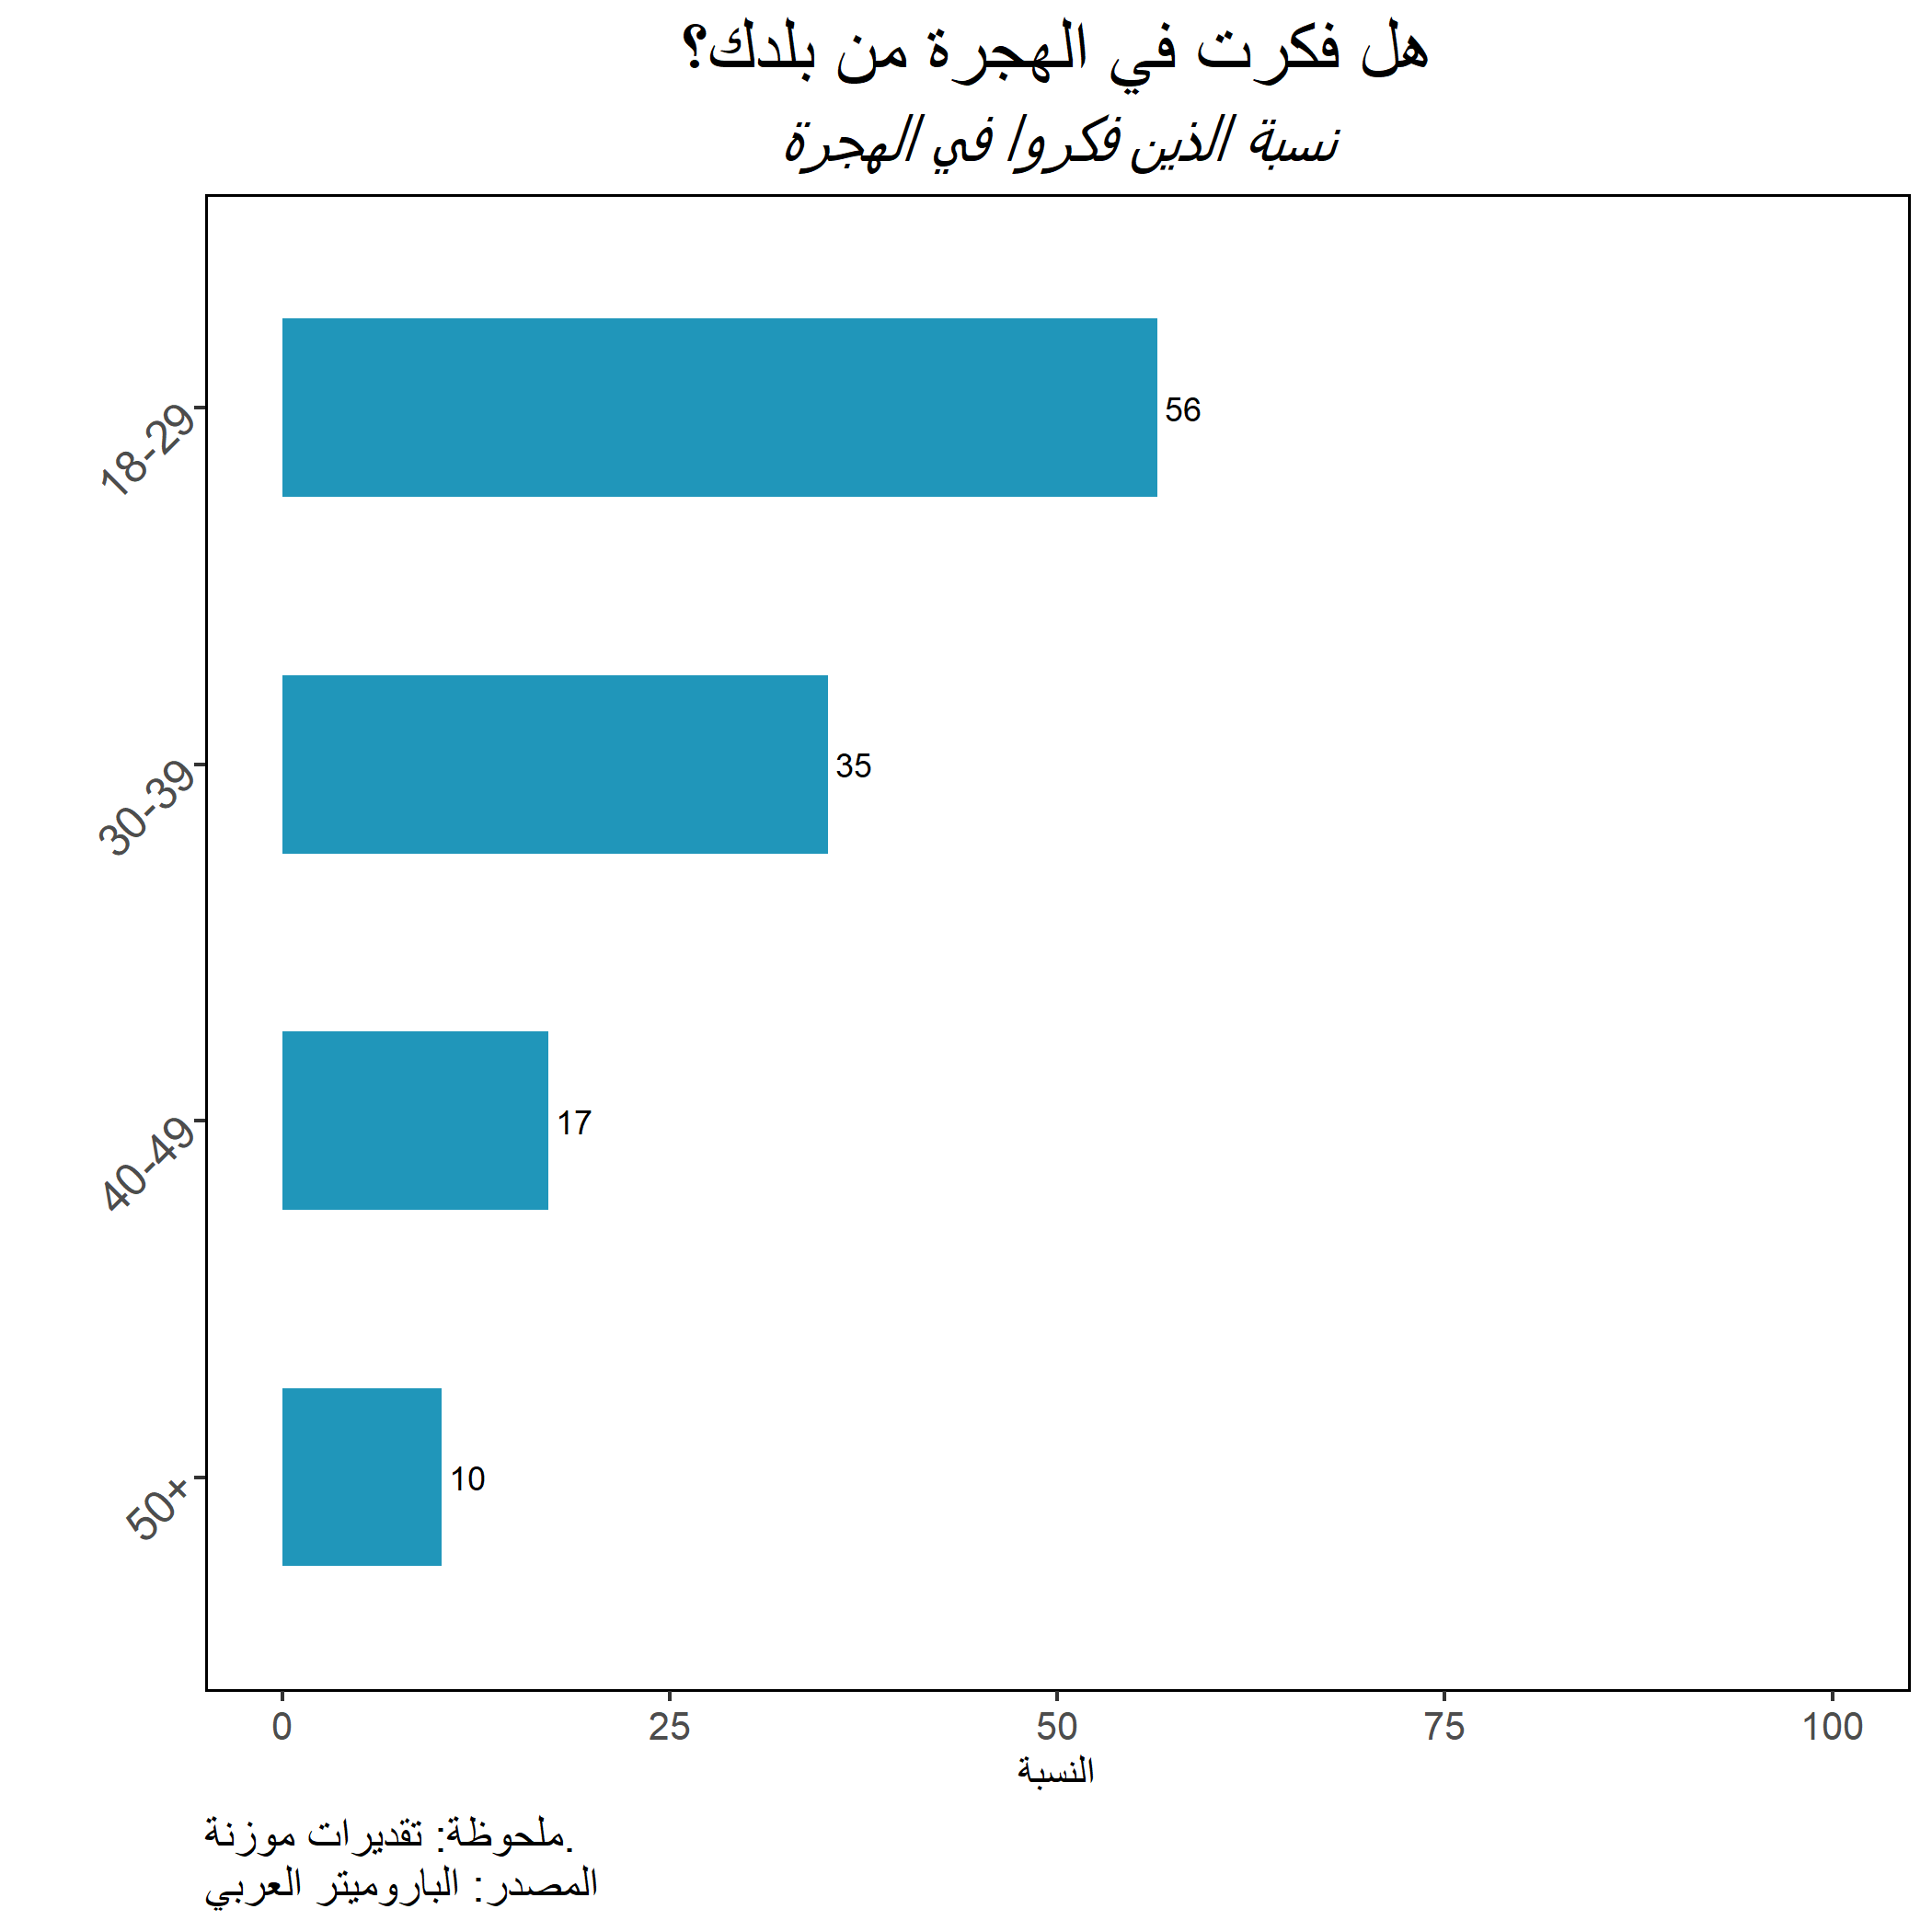
\includegraphics[width=9cm]{Q104_age.png} 
			\end{figure}
	\begin{figure}[H]
	      \centering
				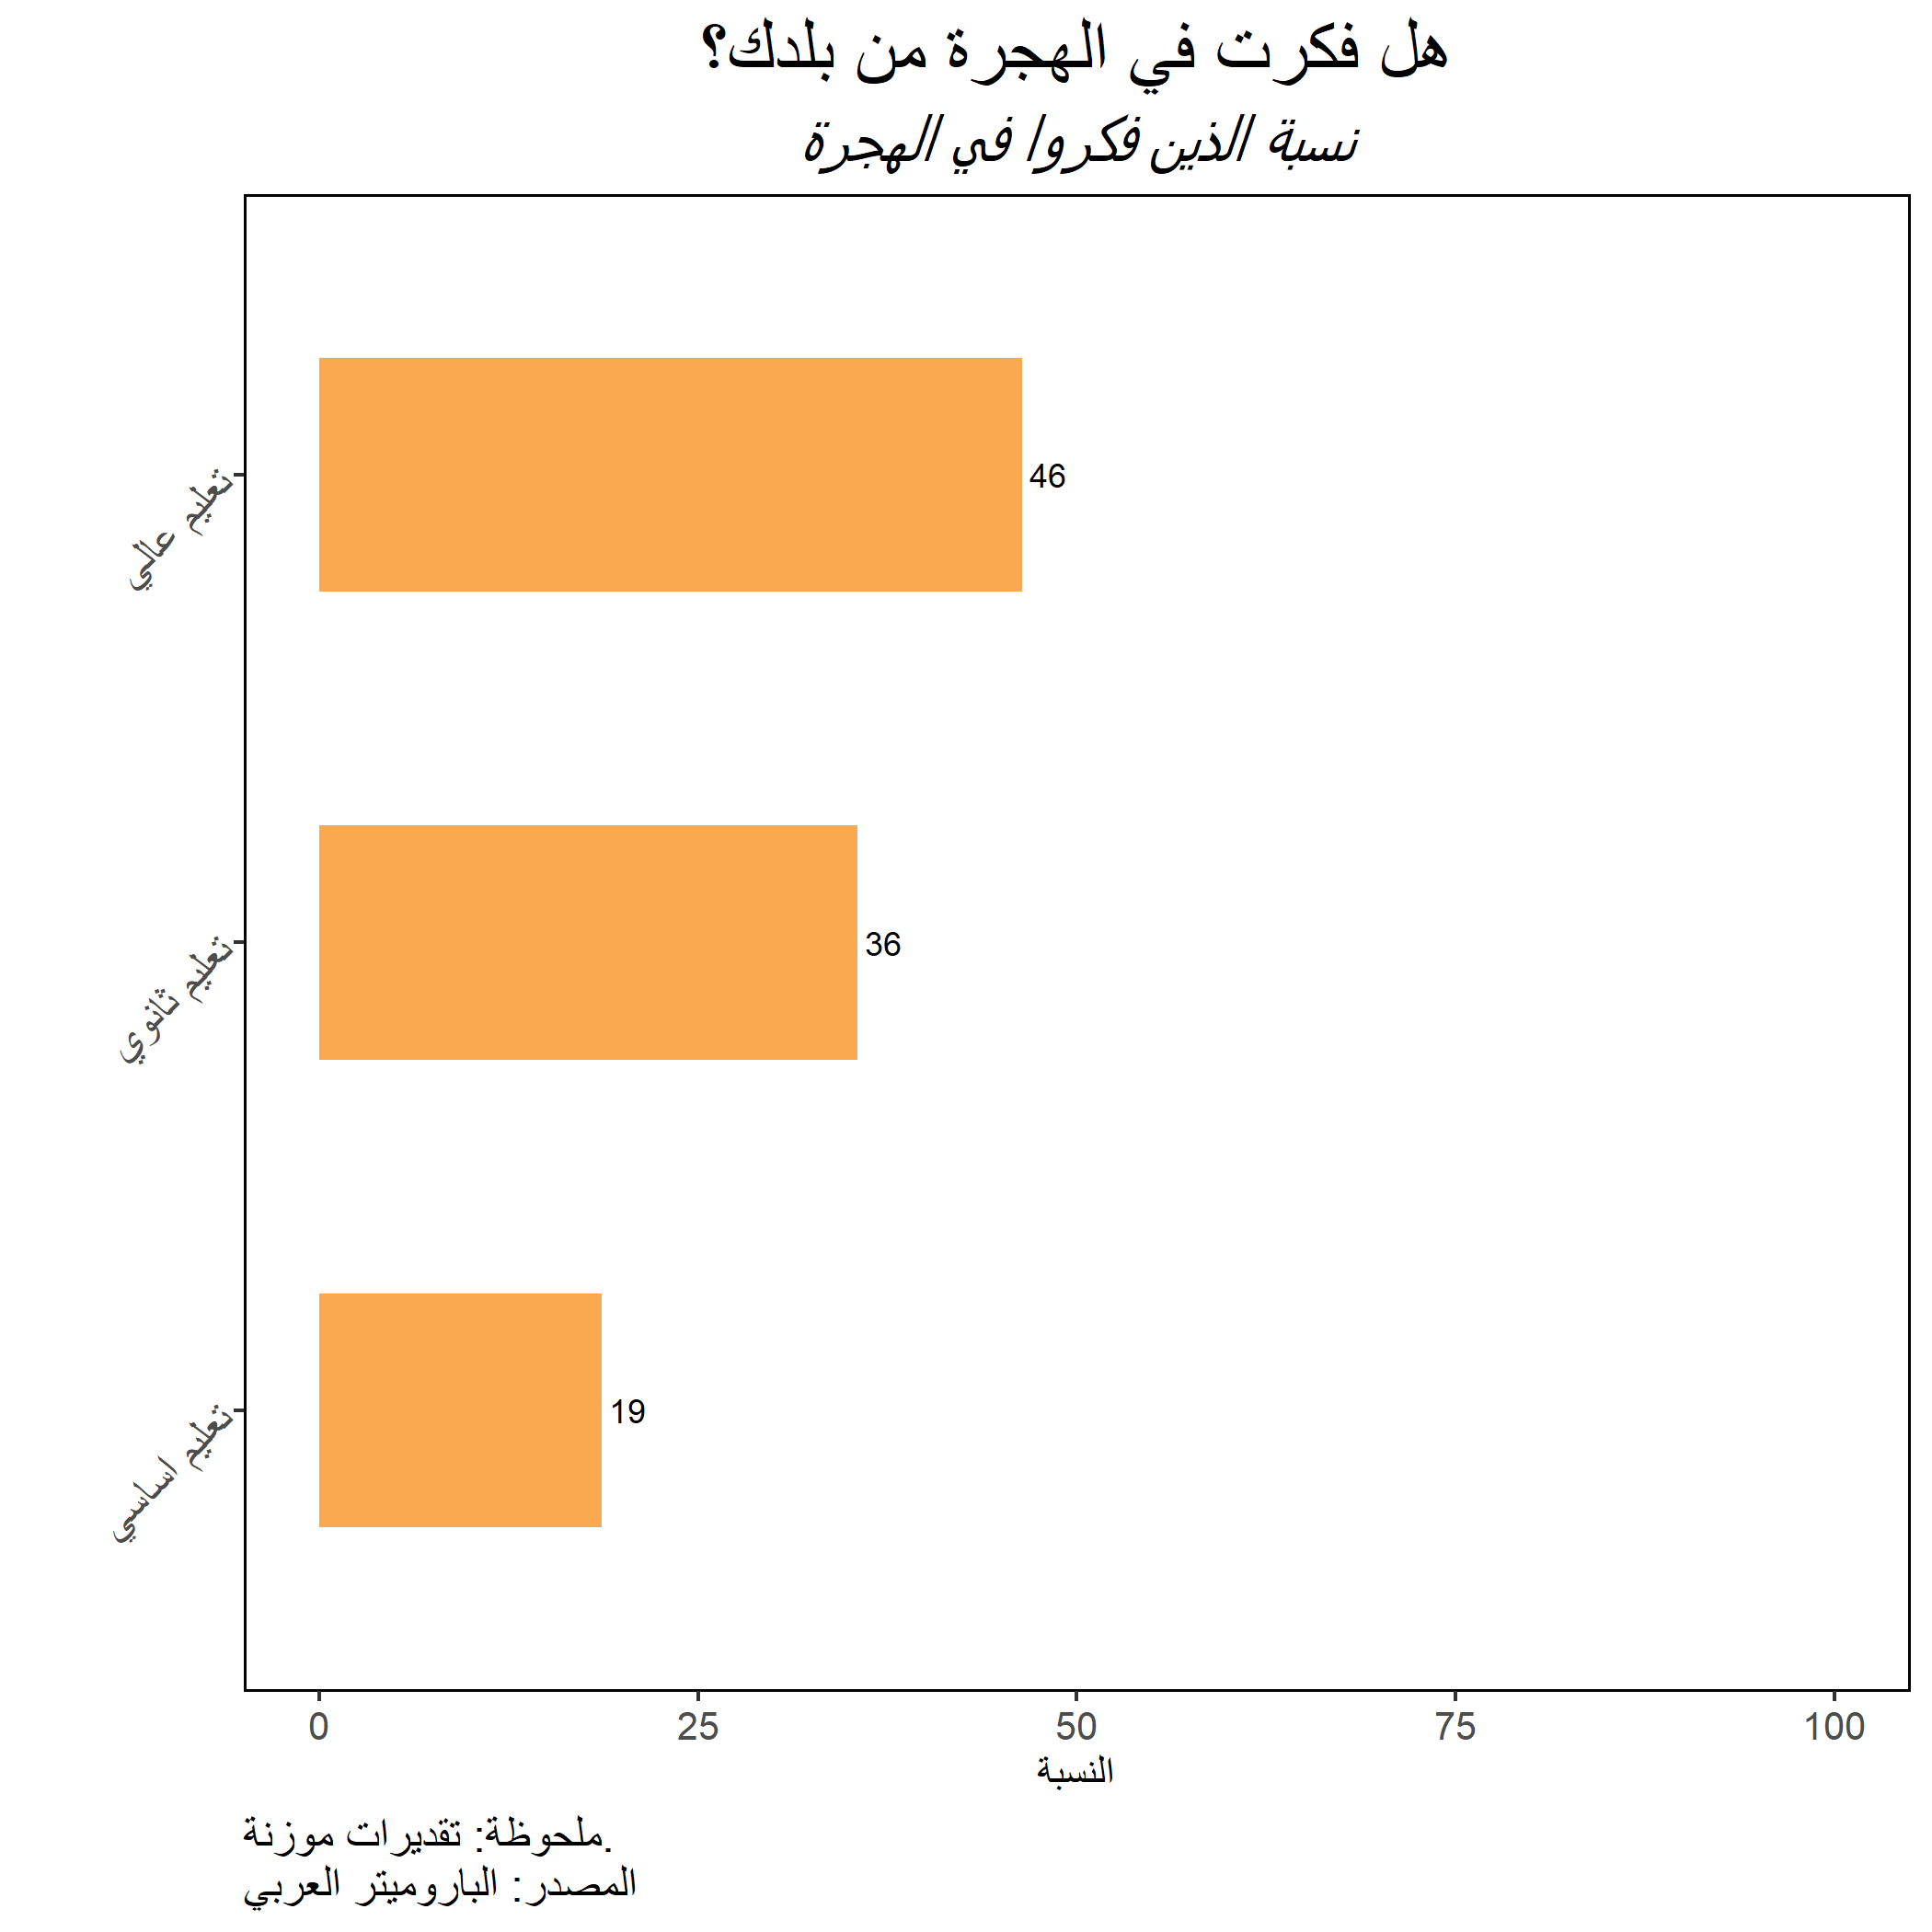
\includegraphics[width=9cm]{Q104_education.png}
			\end{figure}
			
 كما أن الرجال أكثر إقبالاً بكثير من النساء على التفكير في الهجرة (42 بالمئة مقارنة بـ 17 بالمئة)، في حين أن سكان الحضر مقبلون أكثر على الرغبة في الهجرة مقارنة بسكان الريف (7+ نقطة مئوية). ويلاحظ أن سكان منطقة الوسط المحيطة بالجزائر العاصمة يقل إقبالهم على التفكير في الهجرة بواقع 10 نقاط مئوية مقارنة بسكان المناطق الأخرى.
	
 وفي أوساط الراغبين في الهجرة، فإن الأسباب الرئيسية للتفكير فيها تتباين كثيراً. العامل الأكثر شيوعاً هو الأسباب الاقتصادية (38 بالمئة) ثم الفساد (22 بالمئة) والفرص التعليمية (16 بالمئة) ولم شمل الأسرة (10 بالمئة).
	
 طُلب من الراغبين في الهجرة تحديد الأماكن التي يفكرون في الهجرة إليها، بما يشمل إن كان لديهم أكثر من مكان يرغبون في الهجرة إليه. يفكر ثلثا الراغبين في الهجرة من الجزائر في الذهاب إلى أوروبا، في حين أن أكثر من الثلث بقليل (36 بالمئة) ذكروا أمريكا الشمالية. وفي الوقت نفسه فإن شخص واحد من كل 10 أشخاص تقريباً (12 بالمئة) ذكر دول مجلس التعاون الخليجي، في حين يقول 6 بالمئة إنهم يريدون الانتقال إلى دولة أخرى في الشرق الأوسط وشمال أفريقيا غير دول الخليج. ويقول 42 بالمئة من المهاجرين المحتملين إنهم يفكرون في الهجرة غير القانونية.

\section*{الفساد }

 لم يكن ممكناً ضم العديد من الأسئلة عن الفساد في الجزائر من بين الأسئلة التي تم استخدامها في الدورات السابقة. لكن كان من الممكن السؤال عن مدى انتشار دفع الرشاوى في بعض جوانب الحياة اليومية للمواطن.
	
 يقول أغلب الجزائريين (56 بالمئة) إنه من الضروري دفع رشوة لموظف دولة للحصول على خدمات رعاية صحية أفضل. والشباب بين 18 و29 عاماً يقبلون بدرجة أعلى بعض الشيء على القول بأن الرشاوى ضرورية، مقارنة بالأكبر سناً. كما أن سكان الساحل الأوسط حول العاصمة يقبلون أكثر على القول بأن الرشاوى مطلوبة لتحصيل رعاية صحية أفضل، مقارنة بسكان المناطق الأخرى.
	
%	\pagebreak

			\begin{figure}[H]
				\centering
				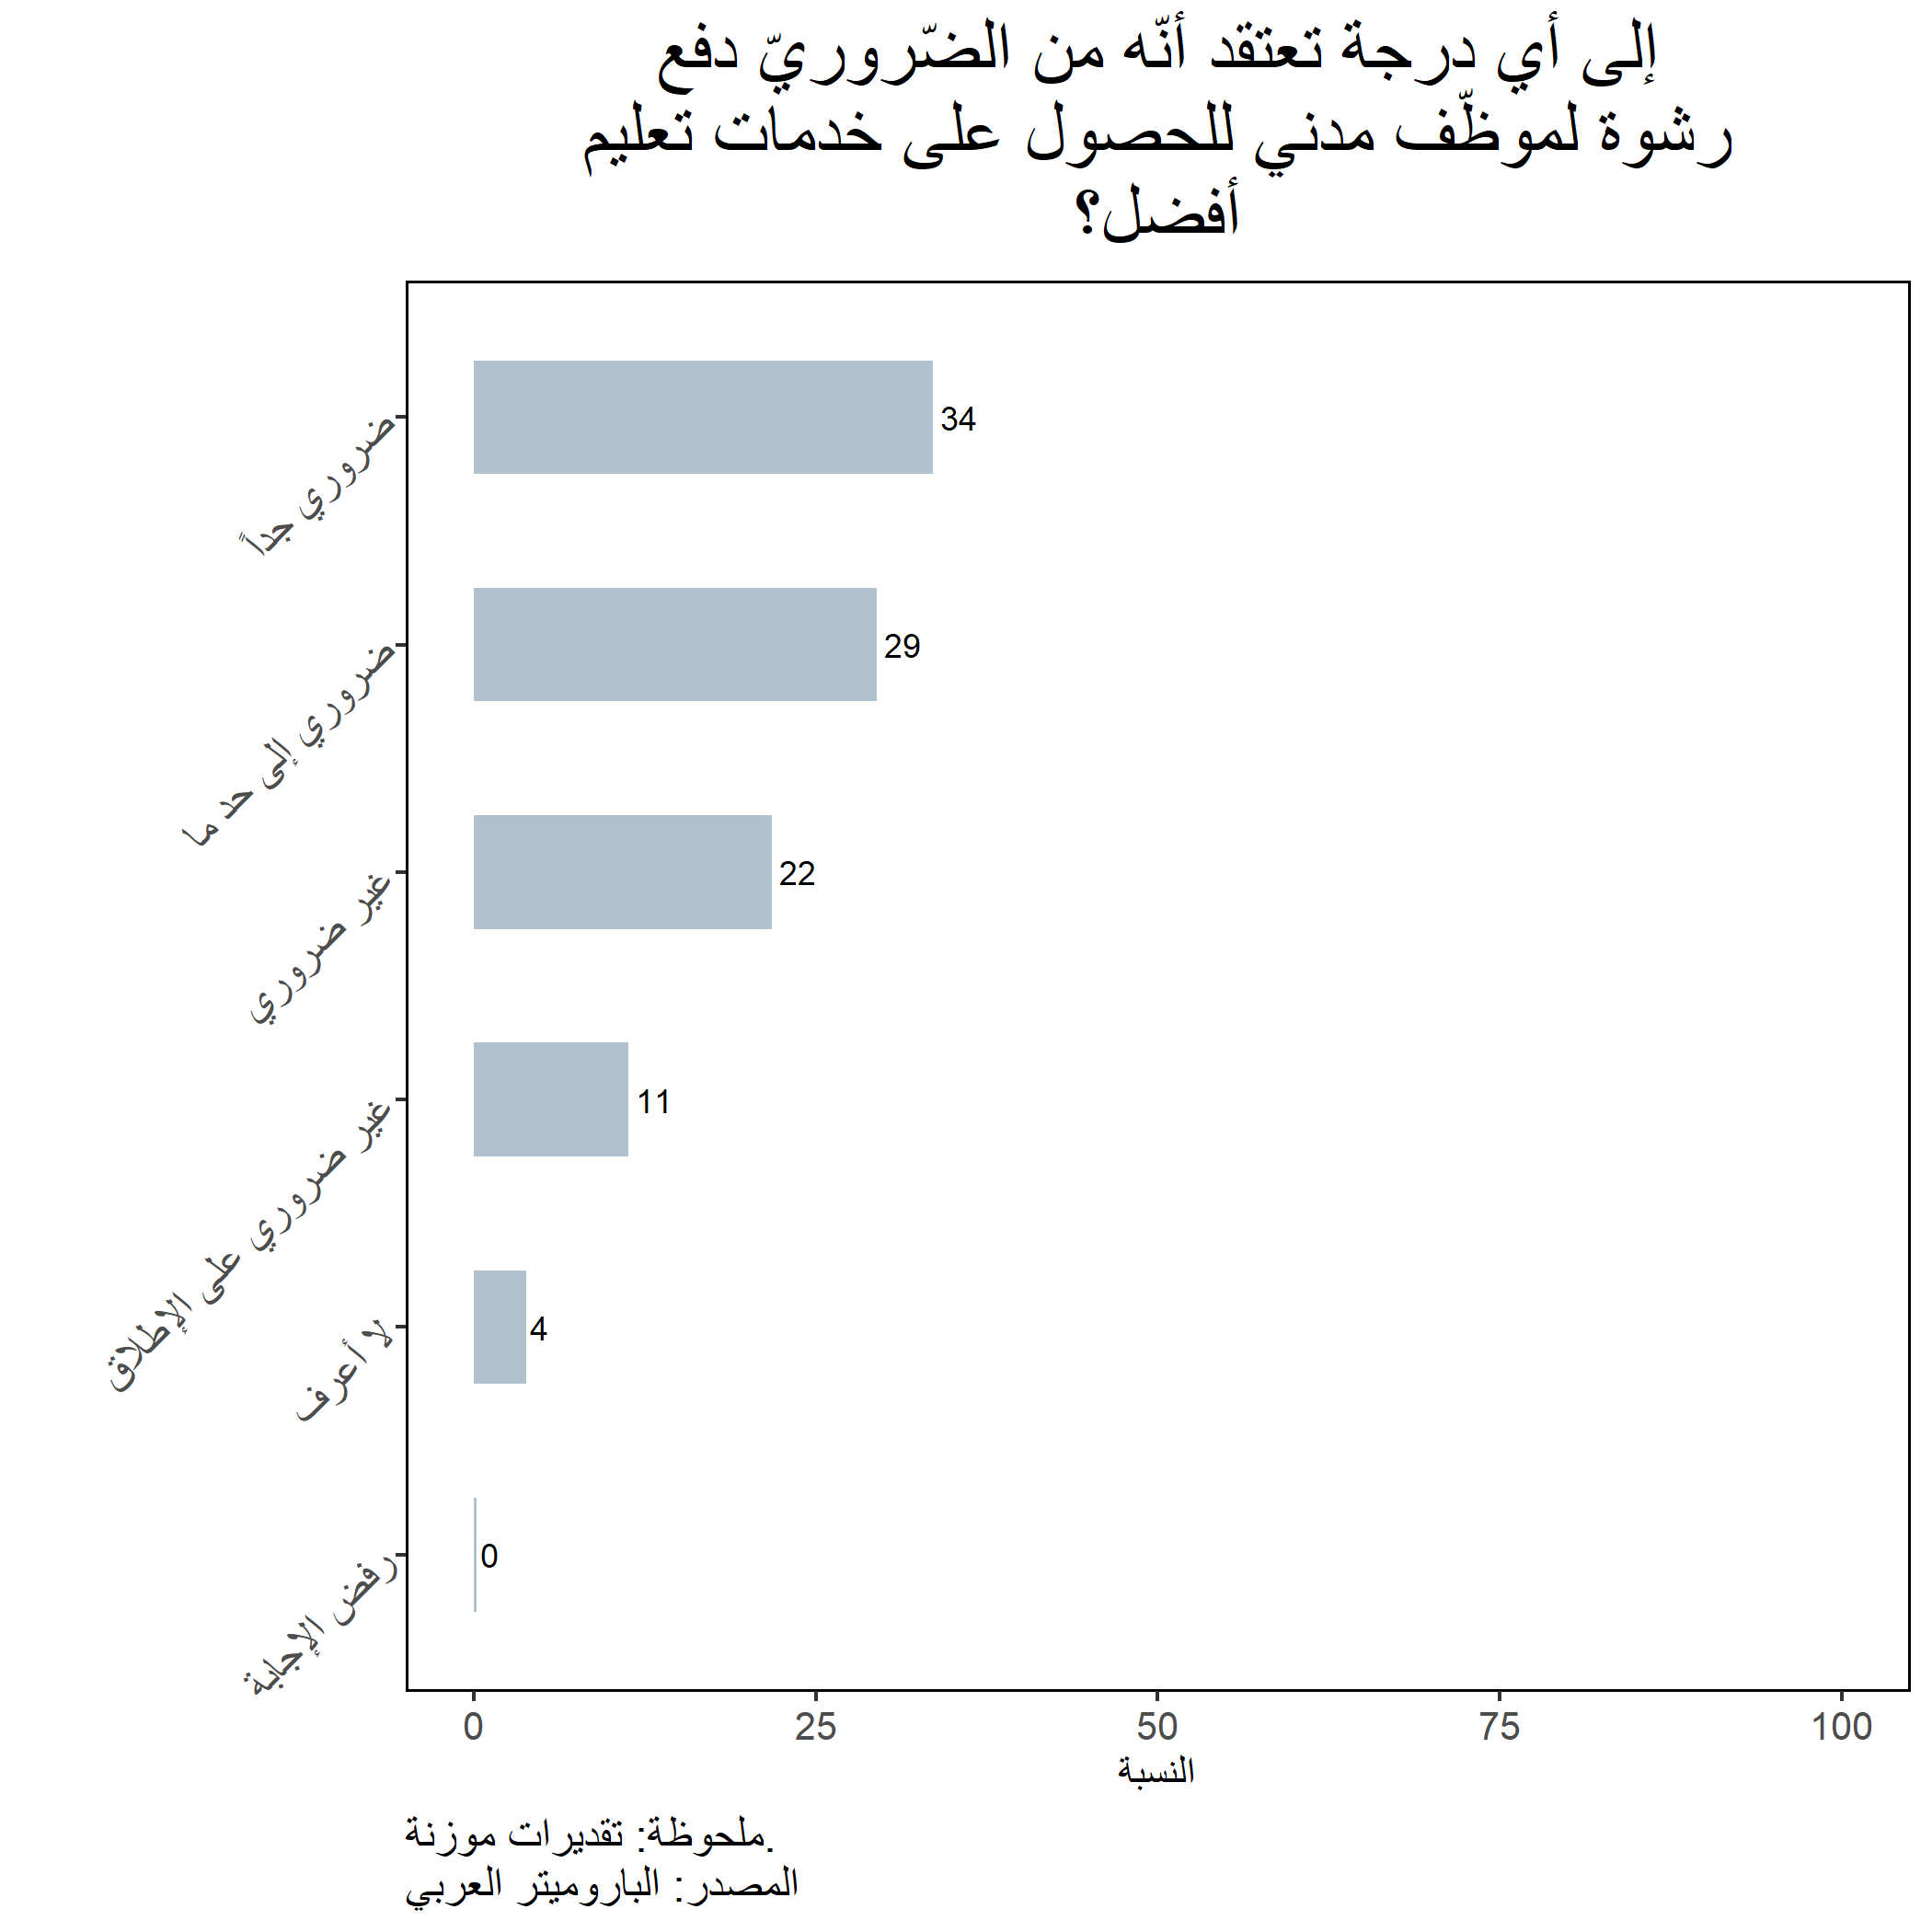
\includegraphics[width=9cm]{Q211b.png} 
			\end{figure}
		
	\begin{figure}[H]
	      \centering
				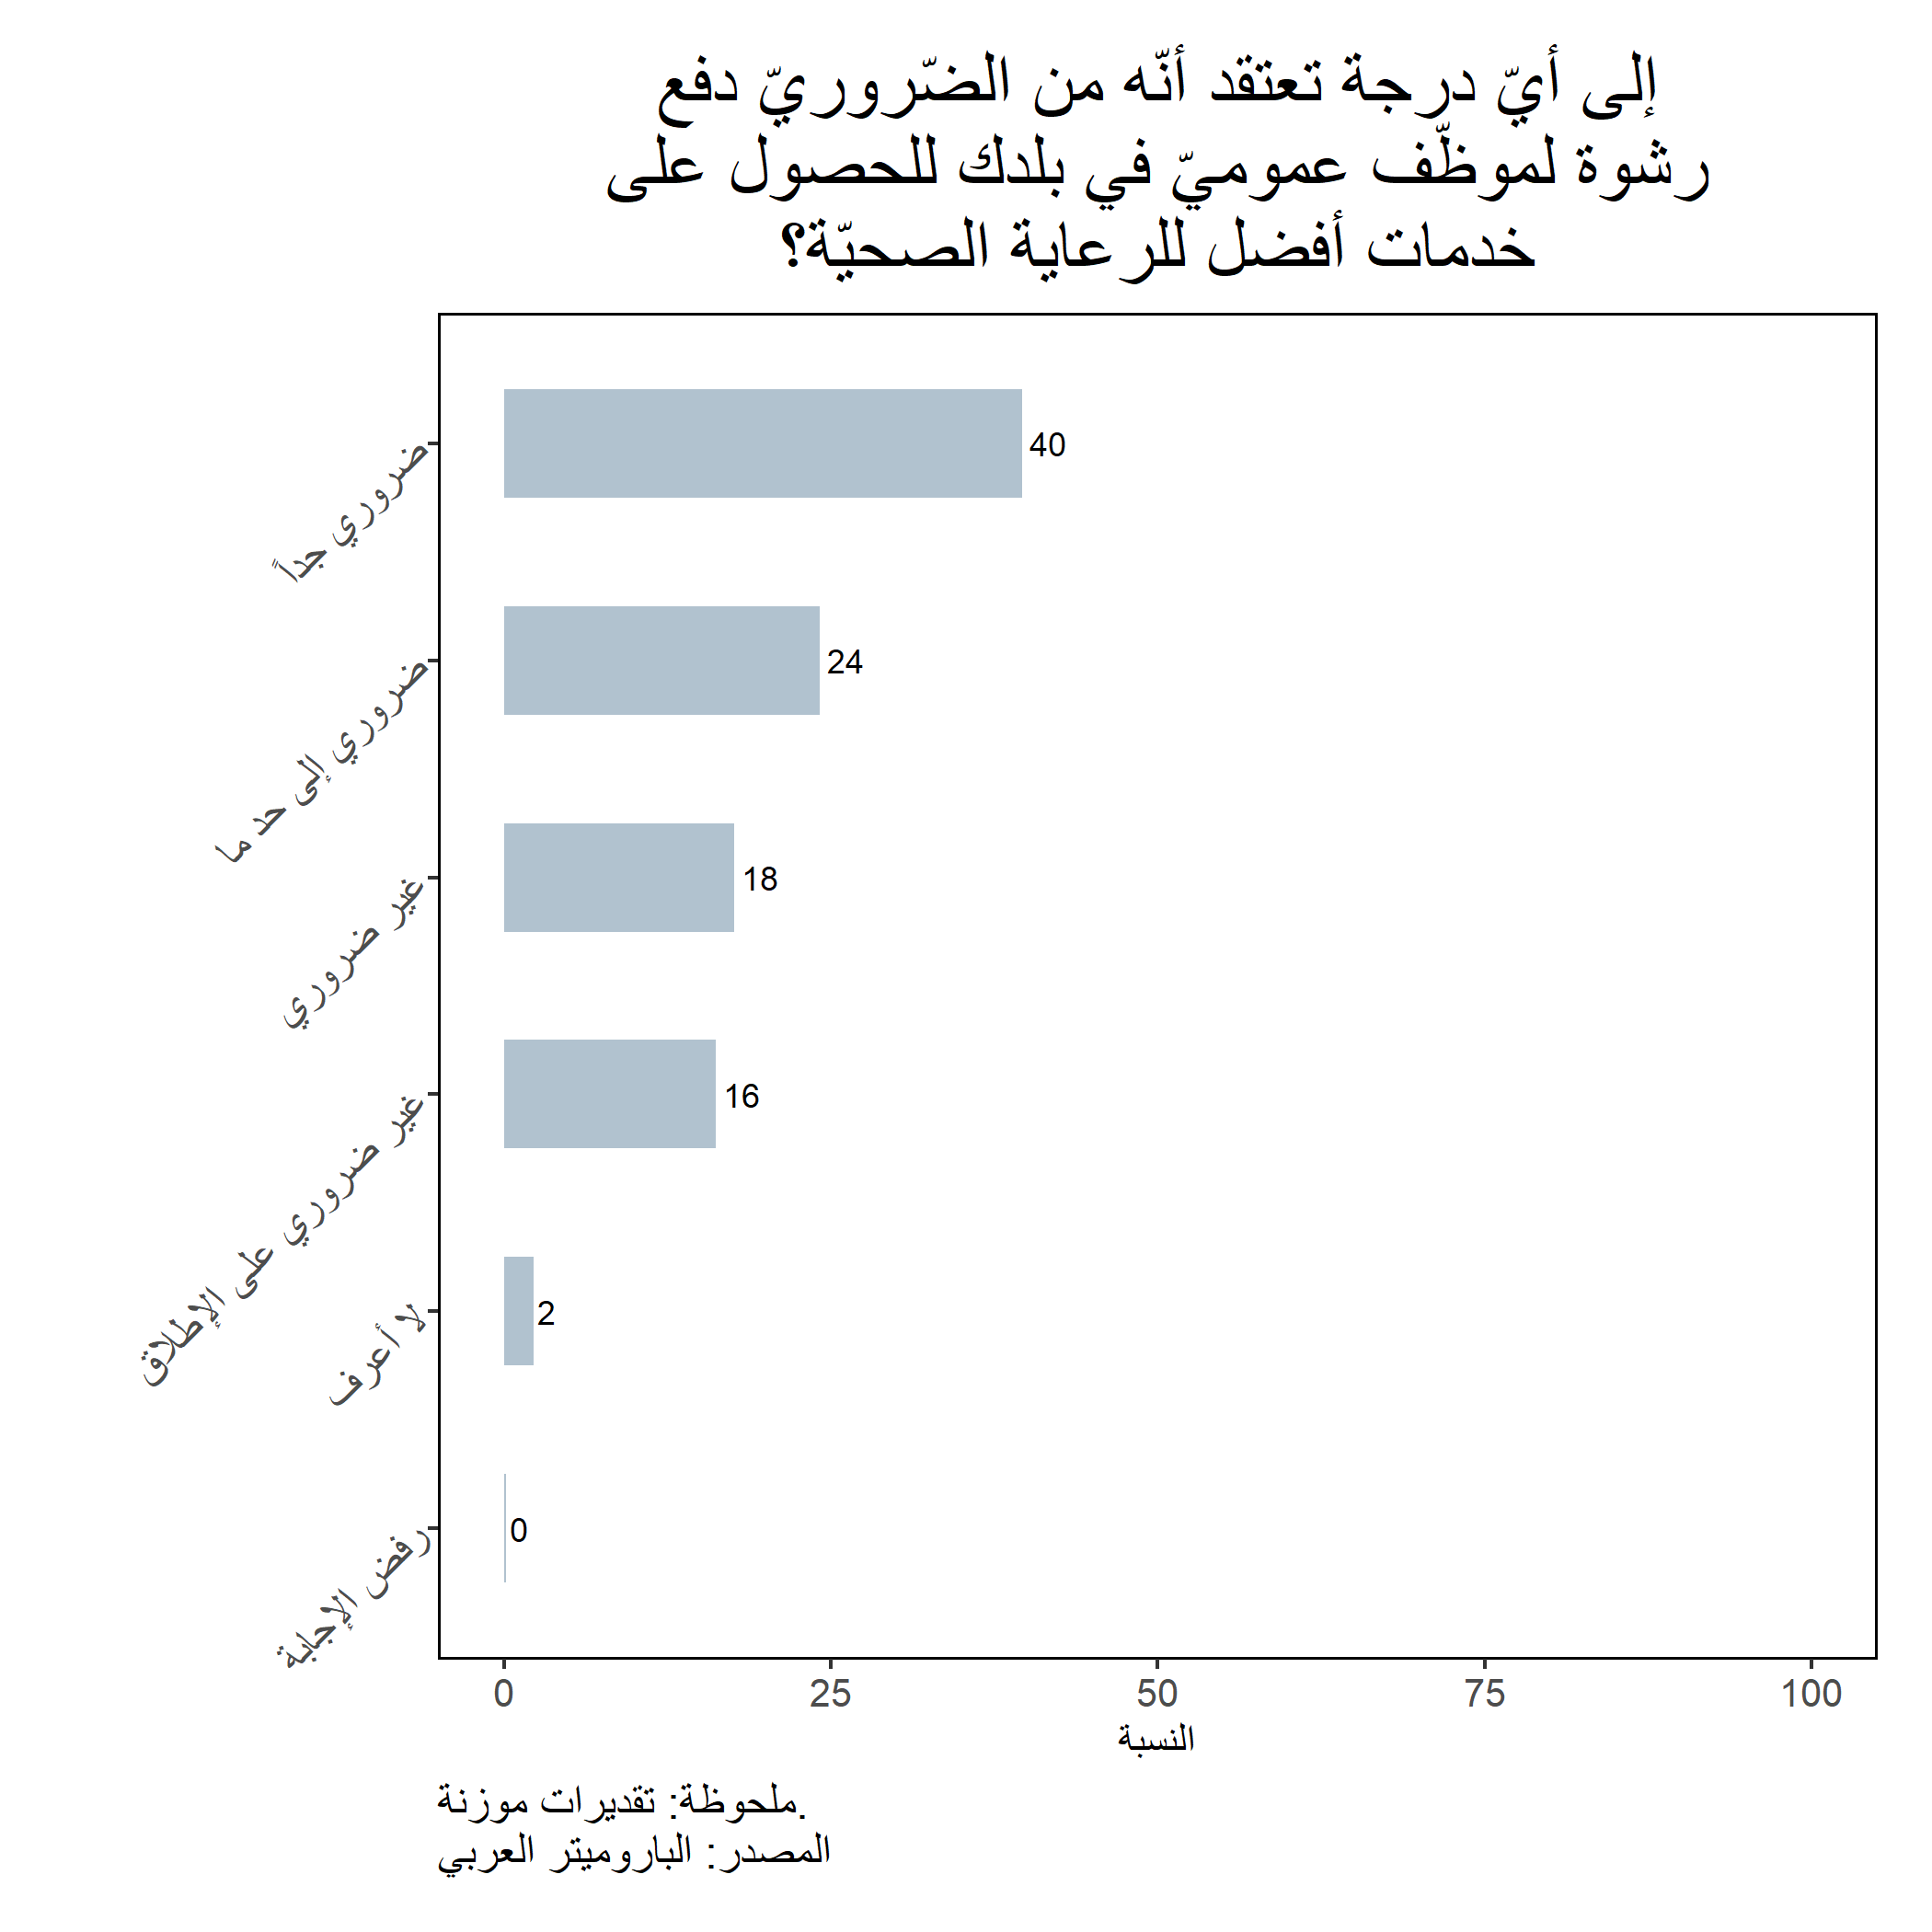
\includegraphics[width=9cm]{Q211c.png}
			\end{figure}
		

 هناك نسبة أصغر لكن ليست بالهينة (45 بالمئة) تقول إنه من الضروري دفع رشوة للحصول على خدمات تعليمية أفضل. والمواطنون الأصغر سناً هم الأكثر إقبالاً على القول بأن الرشوة مطلوبة في التعليم، إذ أن من تتراوح أعمارهم بين 18 و29 عاماً يزيد إقبالهم على هذا الرأي بواقع 15 نقطة مئوية من الذين تبلغ أعمارهم 50 عاماً فأكثر، في حين أن من يعيشون في المناطق الريفية يقبلون على هذا الرأي بواقع 10 نقاط مئوية أكثر من سكان الحضر.
	
\section*{الأداء الحكومي }
	
 يصنف الجزائريون الأداء الحكومي في ملف الاقتصاد بصفته أداءً ضعيفاً. هناك شخص واحد من كل 10 أشخاص يقول إن الحكومة تحسن التعامل مع ملف استحداث الوظائف والحد من التضخم وتقليل أوجه انعدام المساواة. هذه النسب الضئيلة تمثل انحساراً ملحوظاً مقارنة بعام 2013. فالجزائريون الآن أقل إقبالاً بواقع 20 نقطة مئوية على القول بأن الحكومة تحسن استحداث الوظائف و17 نقطة أقل في الاعتقاد بقدرة الحكومة على تقليل أوجه انعدام المساواة، مقارنة بالوضع قبل 6 سنوات. ونظراً لتدني النسب عموماً، فهناك تباين ضئيل بحسب المنطقة الجغرافية، فالجزائريون جميعاً تقريباً يرون أن الأداء الحكومي سيئ للغاية في هذا الجانب.
	
	\pagebreak
	\begin{center}
		\begin{figure}[H]
			\centering
			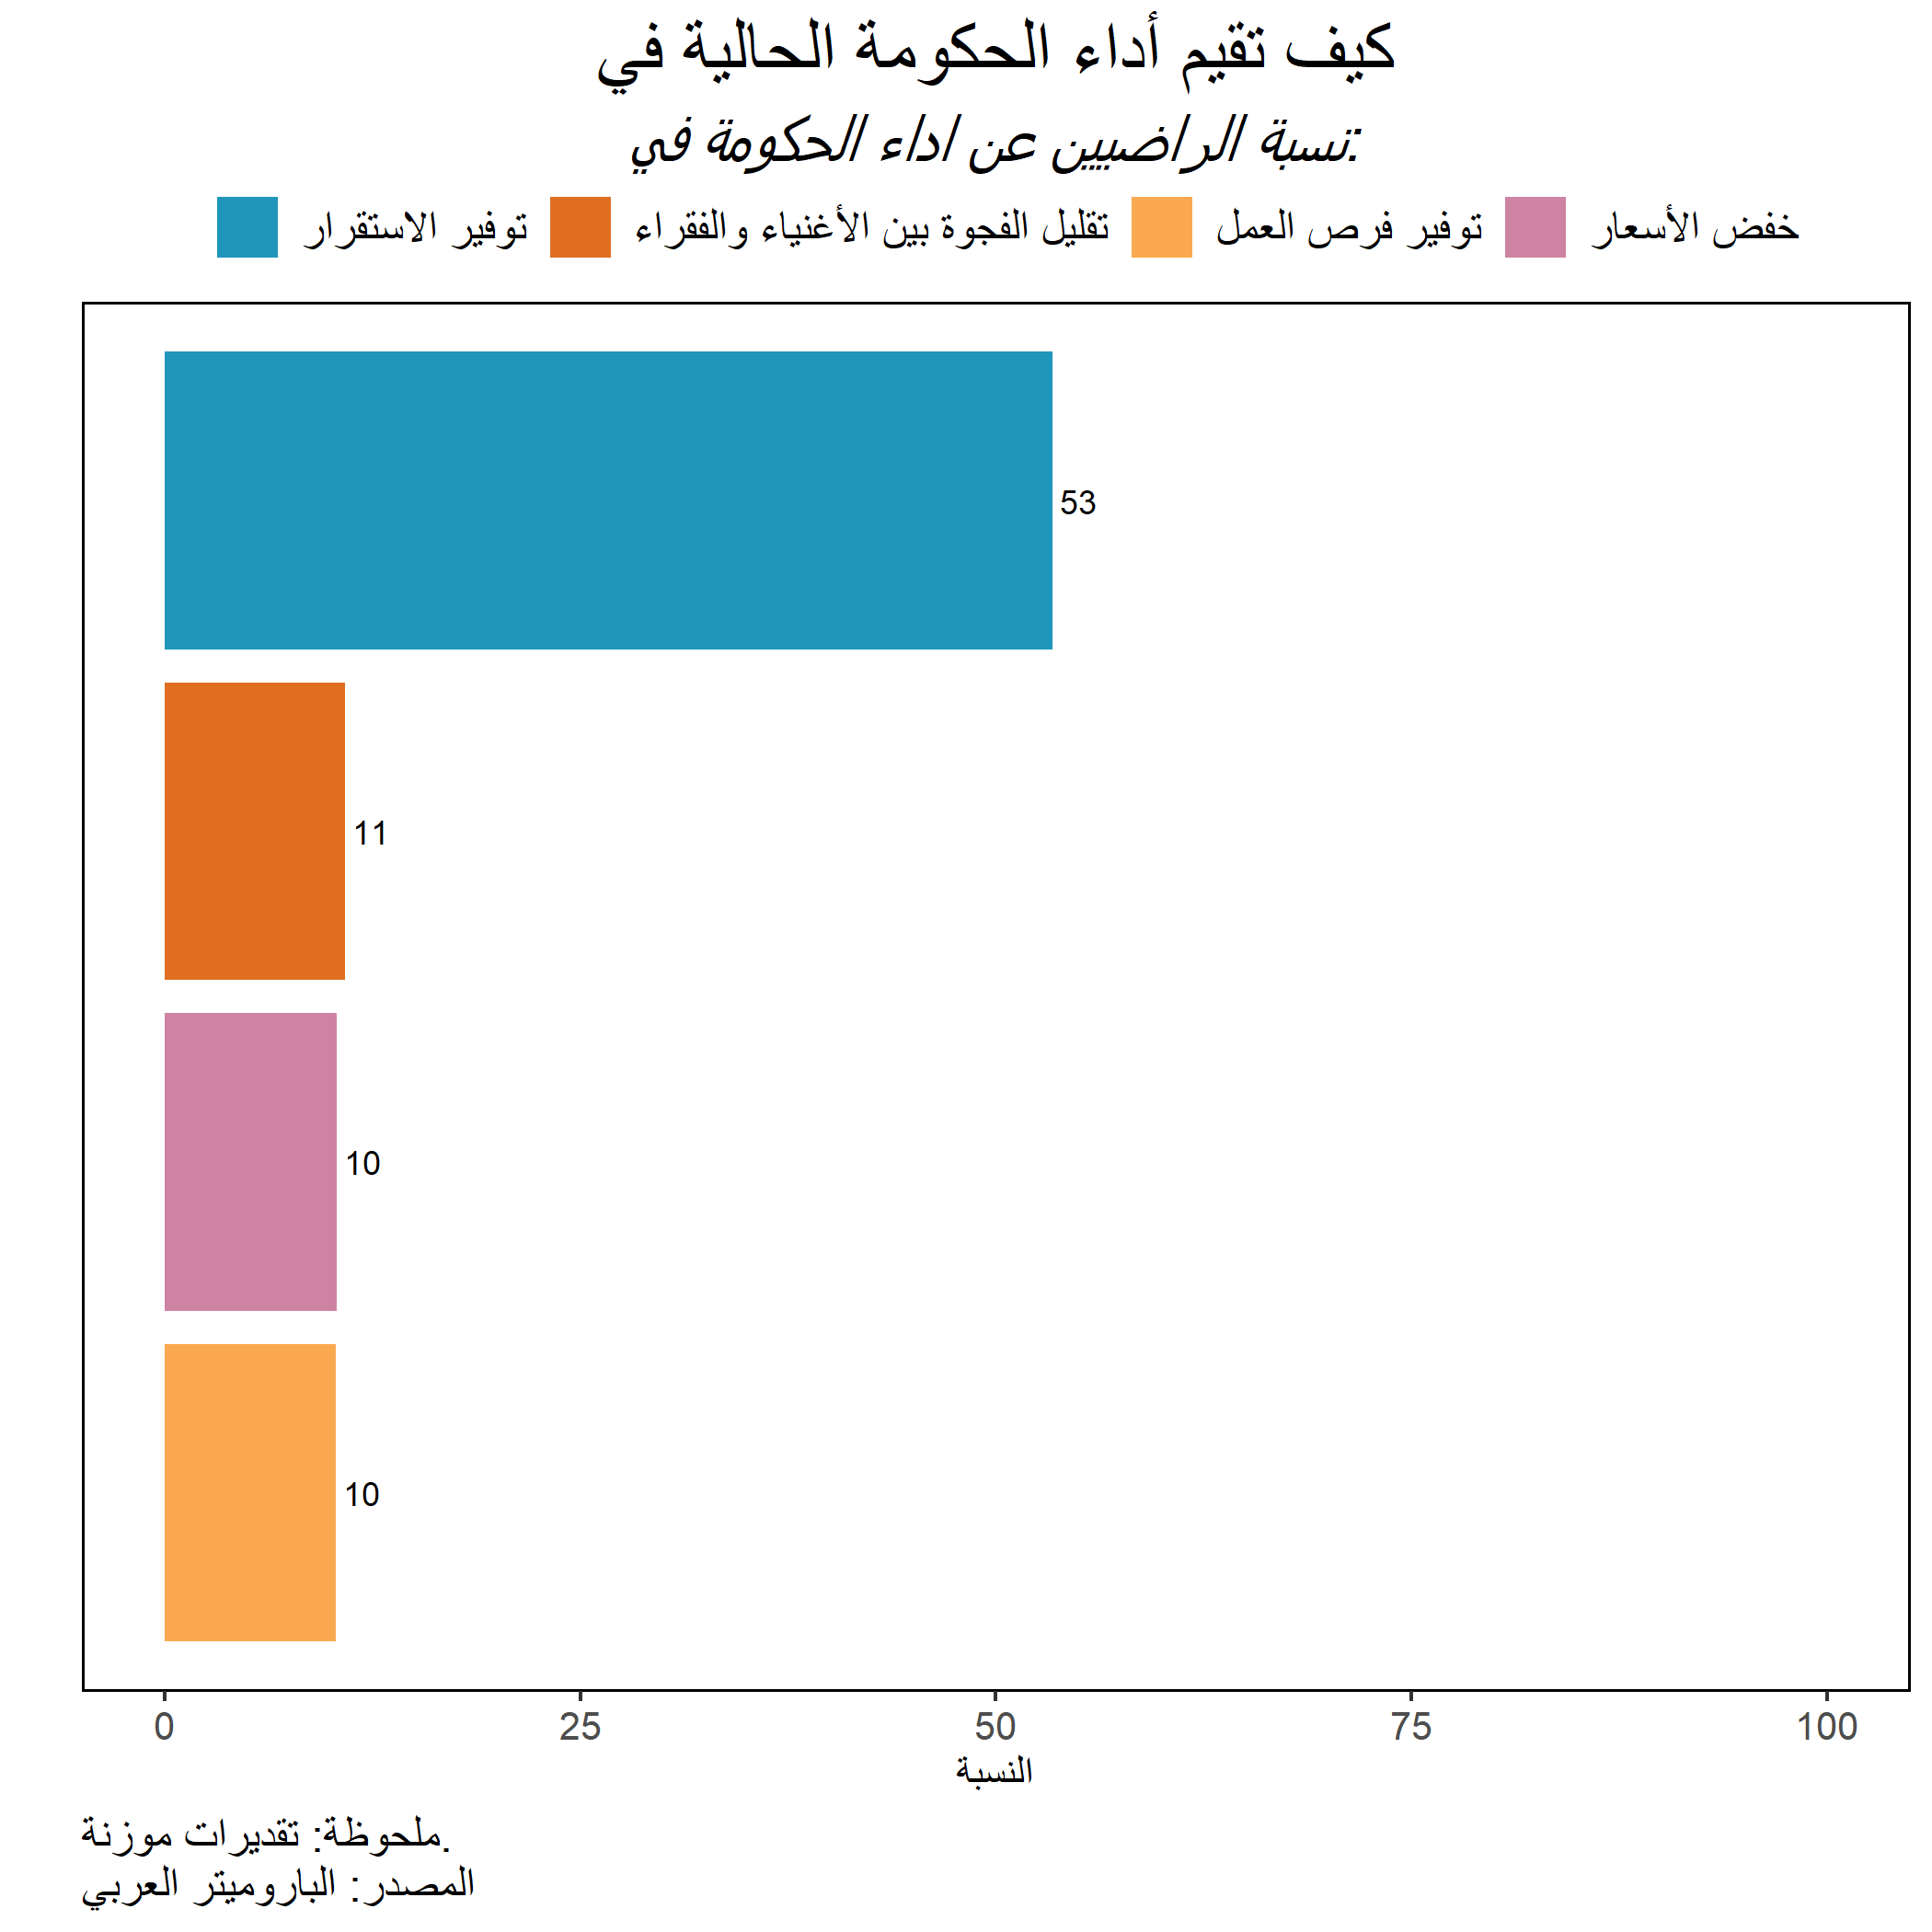
\includegraphics[width=13cm]{Q204.png}
		\end{figure}
	\end{center}
	
 على أن مدركات الأداء الحكومي الخاصة بتوفير الأمن كانت أكثر إيجابية بكثير. إذ أن أكثر من النصف (53 بالمئة) يقولون إن الحكومة تحسن توفير الأمن.  إلا أن هذا المستوى يمثل انحداراً بواقع 14 نقطة مئوية مقارنة بعام 2016. وتتباين المدركات كثيراً بحسب المنطقة. فنحو ثلاثة أرباع (72 بالمئة) سكان المناطق المحيطة بالعاصمة يقولون إن الحكومة تحسن توفير الأمن في تلك المنطقة، مقارنة بـ 56 بالمئة من سكان شمال غرب الجزائر و38 بالمئة من سكان الشمال الشرقي.
	
 كما كانت الآراء حول جودة الخدمات الأساسية سلبية نسبياً بدورها. فنحو الثلث يقولون إنهم راضون عن النظام التعليمي (36 بالمئة) والرعاية الصحية (31 بالمئة). ويلاحظ أن جودة الخدمات تبدو أعلى في نظر سكان منطقة العاصمة والمناطق المحيطة، مقارنة بمناطق الجزائر الأخرى، إذ أن من يعيشون في المنطقة الساحلية الوسطى هم الأكثر إقبالاً على تصنيف خدمات التعليم والصحة بصورة إيجابية.
	
\section*{التفضيلات السياسية }
	
 دعم الديمقراطية مختلط في الجزائر. فلدى سؤالهم، وافق نحو 4 من كل 10 أشخاص (41 بالمئة) على أن الديمقراطية هي النظام الأفضل دائماً، وهي من أقل النسب في المنطقة من بين الدول المشمولة بالاستطلاع. وفي الوقت نفسه يقول 3 من كل 10 أشخاص إن الحكومة غير الديمقراطية تكون أفضل أحياناً، في حين أن الخُمس (21 بالمئة) يقولون إنه لا يهم شكل الحكومة. ودعم الديمقراطية متصل بمستوى التعليم، إذ أن النصف (51 بالمئة) من الحاصلين على شهادة جامعية يفضلون الديمقراطية في كل الأحوال، مقارنة بنحو الثلث (35 بالمئة) من أصحاب التعليم الأساسي.
	
 على أن فهم الجزائريين للديمقراطية يختلف عن الفهم الشائع في الغرب. فلدى سؤالهم عن السمة الأهم للديمقراطية، أجاب 4 من كل 10 أشخاص بأنها ضمان الحكومة للقانون والنظام، وهو ما يُرجح كونه يعكس مخاوف عودة فترة الحرب الأهلية التي اندلعت في التسعينيات. وفي الوقت نفسه فإن الربع تقريباً يقولون إن التعريف الرئيسي للديمقراطية هو أن يكون الإعلام حر في انتقاد الحكومة (23 بالمئة) أو أن تضمن الحكومة فرص العمل للجميع (22 بالمئة). وفي الوقت نفسه يُعرّف شخص واحد من كل 10 أشخاص (9 بالمئة) الديمقراطية من حيث إمكانية عقد انتخابات تتنافس فيها أحزاب متعددة.
	
 وهناك قلة نسبية ترى أن الجزائر ديمقراطية، إذ أن الربع تقريباً (24 بالمئة) يقولون إن الجزائر أقرب للديمقراطية عن الديكتاتورية. والمواطنون المقيمون في العاصمة وحولها هم الأكثر إقبالاً على القول بأن الجزائر ديمقراطية (39 بالمئة)، ومن يعيشون في الشمال الغربي (26 بالمئة) والشمال الشرقي (13 بالمئة) أقل إقبالاً بكثير على هذا الرأي. كما أن 17 بالمئة فقط من الشباب بين 18 و29 عاماً يقولون إن بلدهم ديمقراطي، وهي نسبة أقل مقارنة بالشرائح العمرية الأخرى.
	
	\begin{center}
		\begin{figure}[H]
			\centering
			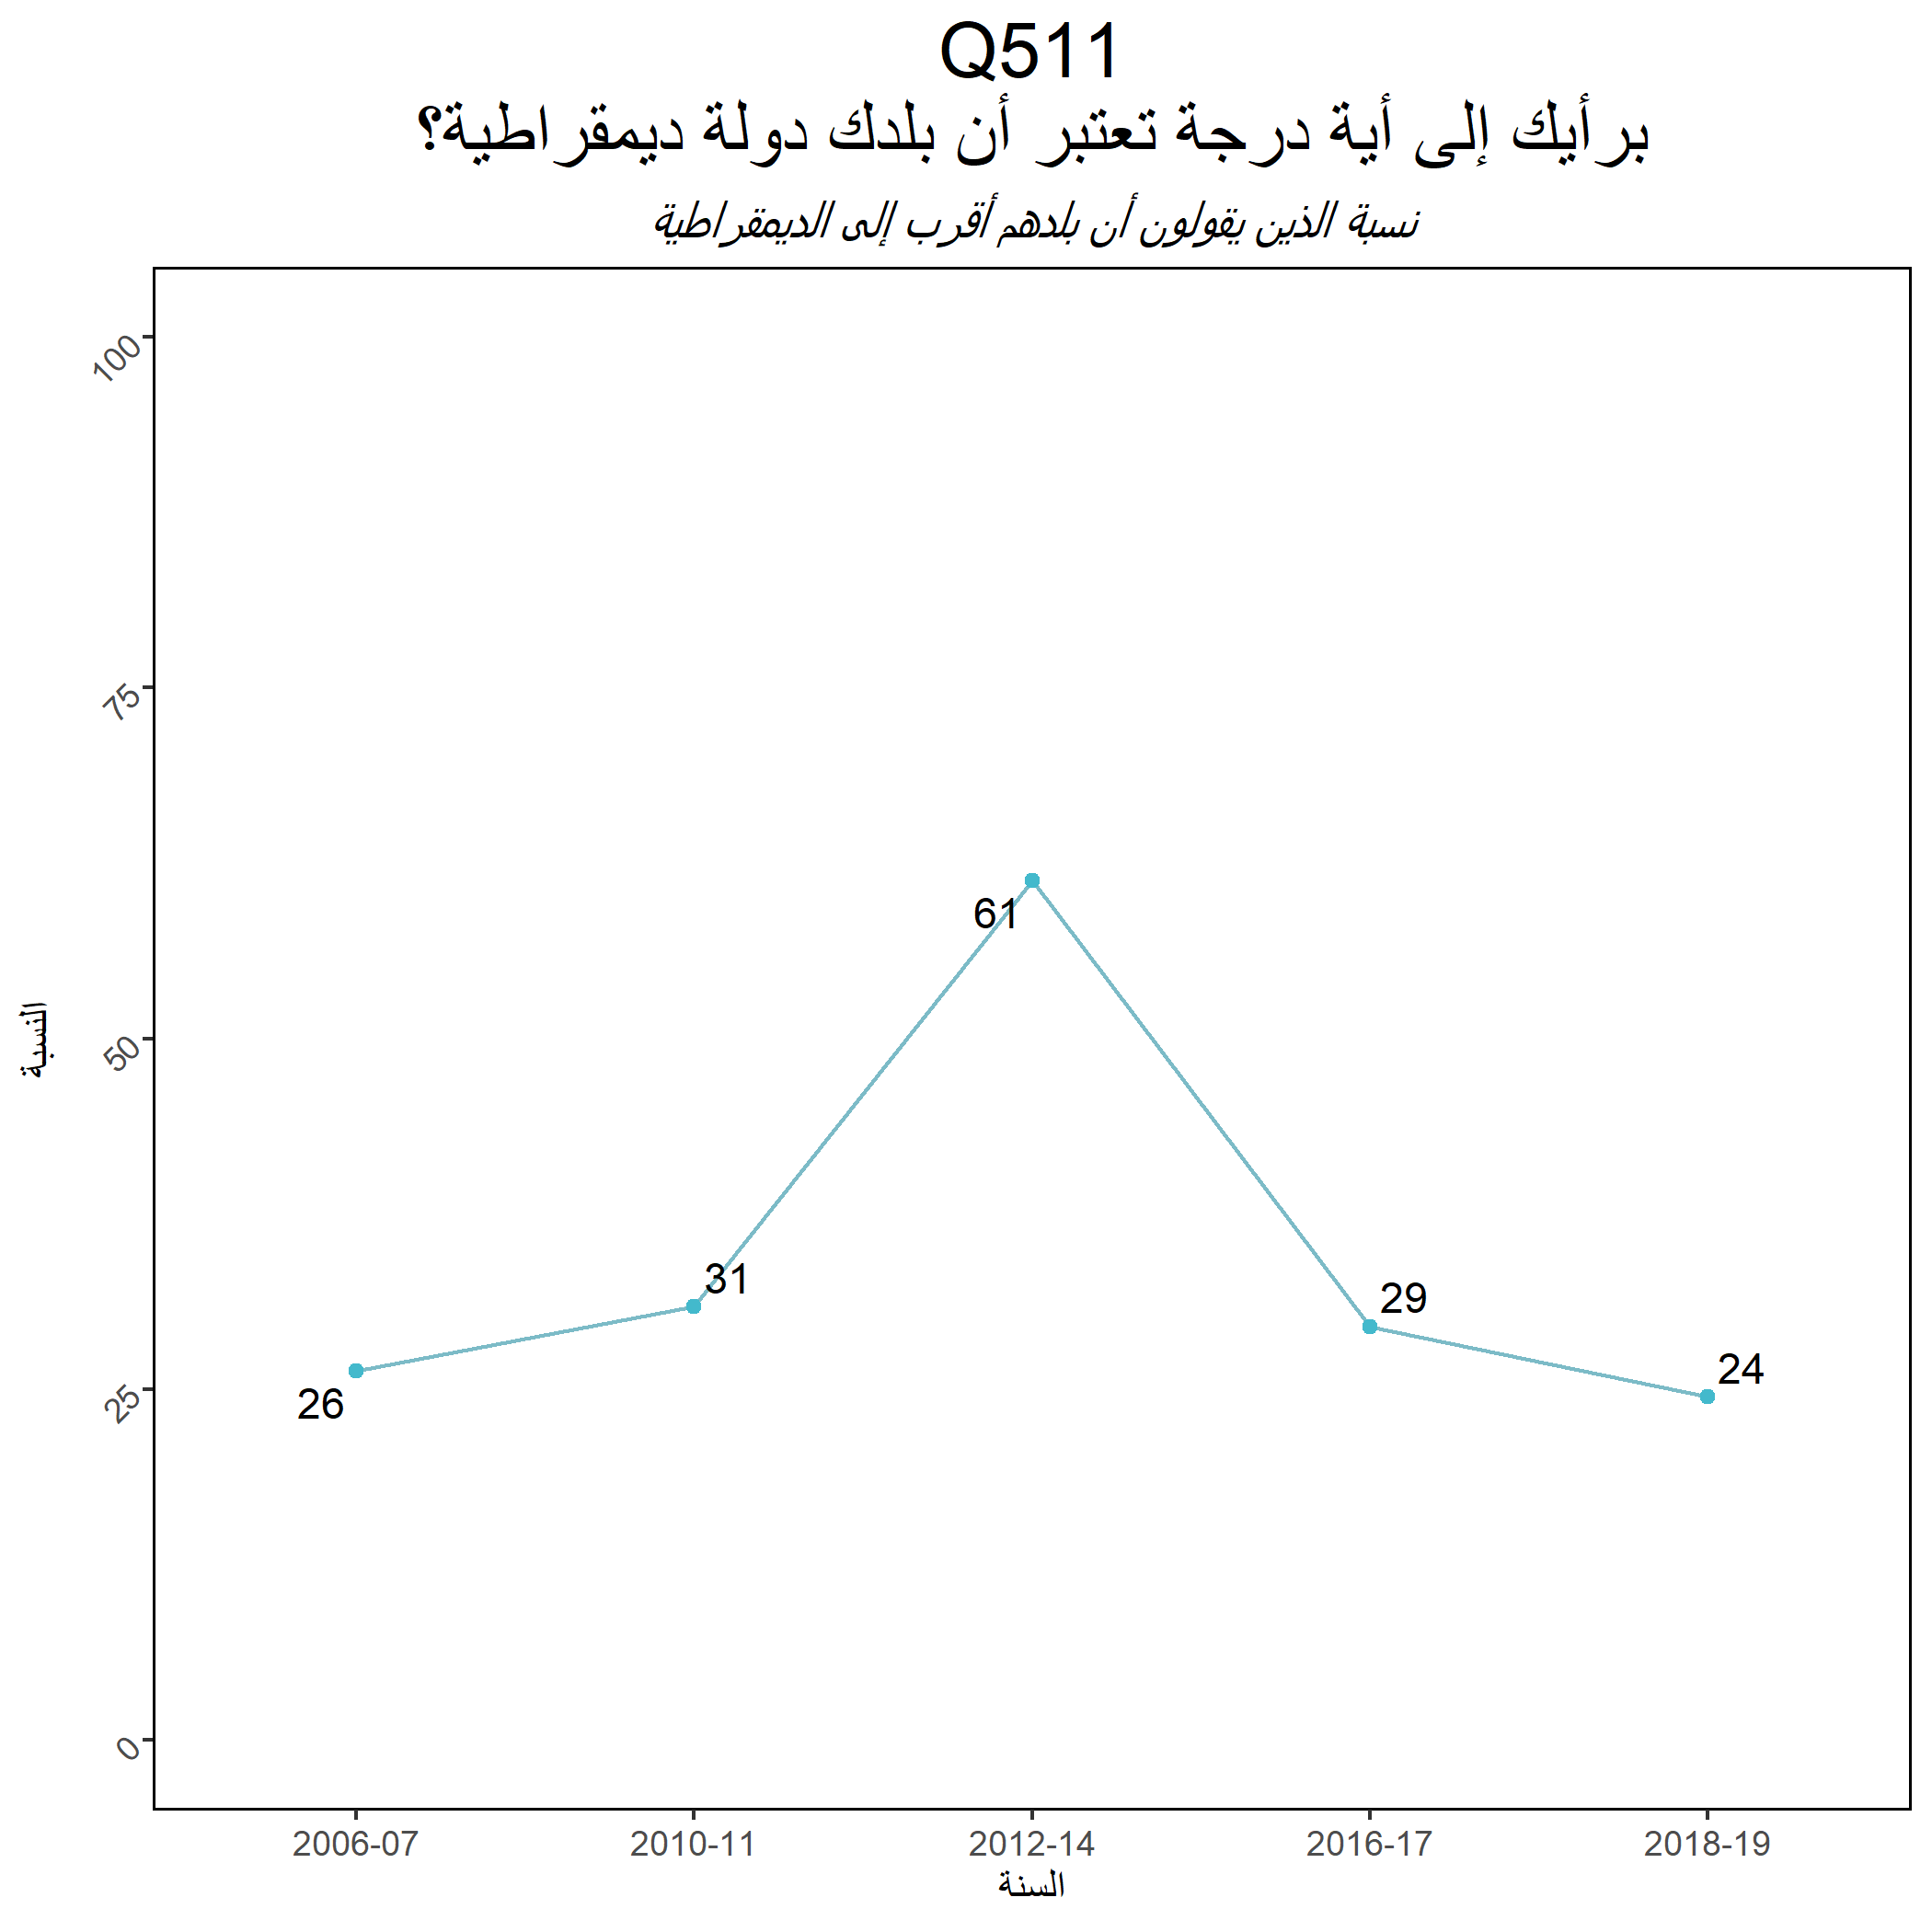
\includegraphics[width=13cm]{Q511_.png}
		\end{figure}
	\end{center}
	
 على الرغم من أن أغلب الجزائريين لا يؤمنون بأنهم يعيشون في نظام ديمقراطي، فهناك أغلبية بسيطة ترى أن هذا النظام السياسي مناسب أكثر لبلدهم مقارنة بنظم أخرى، وهي النسبة التي زادت 11 نقطة مئوية منذ 2016. ويلاحظ أن هذا الرأي يعتنقه من أجري معهم الاستطلاع بالتساوي عبر مختلف الشرائح العمرية ومستويات التعليم.
	
 ورغم قول العديد من الجزائريين إن الديمقراطية مناسبة، فهناك نسبة لا يستهان بها أعربت عن القلق من هذا النظام. على سبيل المثال فإن 4 من كل 10 أشخاص (38 بالمئة) يقولون إن الأداء الاقتصادي يكون سيئاً في النظام الديمقراطي، وهي النسبة التي زادت 22 نقطة مئوية منذ 2013. وبالمثل، فإن 35 بالمئة يقولون إن النظم الديمقراطية غير حاسمة، في حين يقول 3 من كل 10 أشخاص إن النظم الديمقراطية غير فعالة في حفظ النظام، وهي النسبة التي زادت كثيراً منذ عام 2013. يرجح أن هذه التغيرات هي نتيجة لتفكير الجزائريين وتدبّرهم لتجربة تونس المجاورة، حيث واجه الانتقال الديمقراطي عدداً كبيراً من التحديات منذ عام 2011.
	
\section*{الدين والسياسة }

 اندلعت الحرب الأهلية الجزائرية في التسعينيات بعد إلغاء الجيش للجولة الثانية من انتخابات 1990-1991. كانت النتيجة هي نزاع شهد مقتل أكثر من 100 ألف شخص وهزيمة التمرد الإسلامي.
	
 وبعد عقدين تقريباً من انتهاء النزاع، فلا يزال الانقسام الواضح في الجزائر قائماً، حول دور الدين في السياسة. لدى طرح سؤال عما إذا كانت البلاد ستصبح أفضل حالاً إذا شغل أشخاص متدينون أكثر مناصب عامة، أيد 44 بالمئة المقولة، مقارنة بـ 45 بالمئة اختلفوا معها، وهي النسب التي لم تتغير منذ عام 2013.
	
	\begin{center}
		\begin{figure}[H]
			\centering
			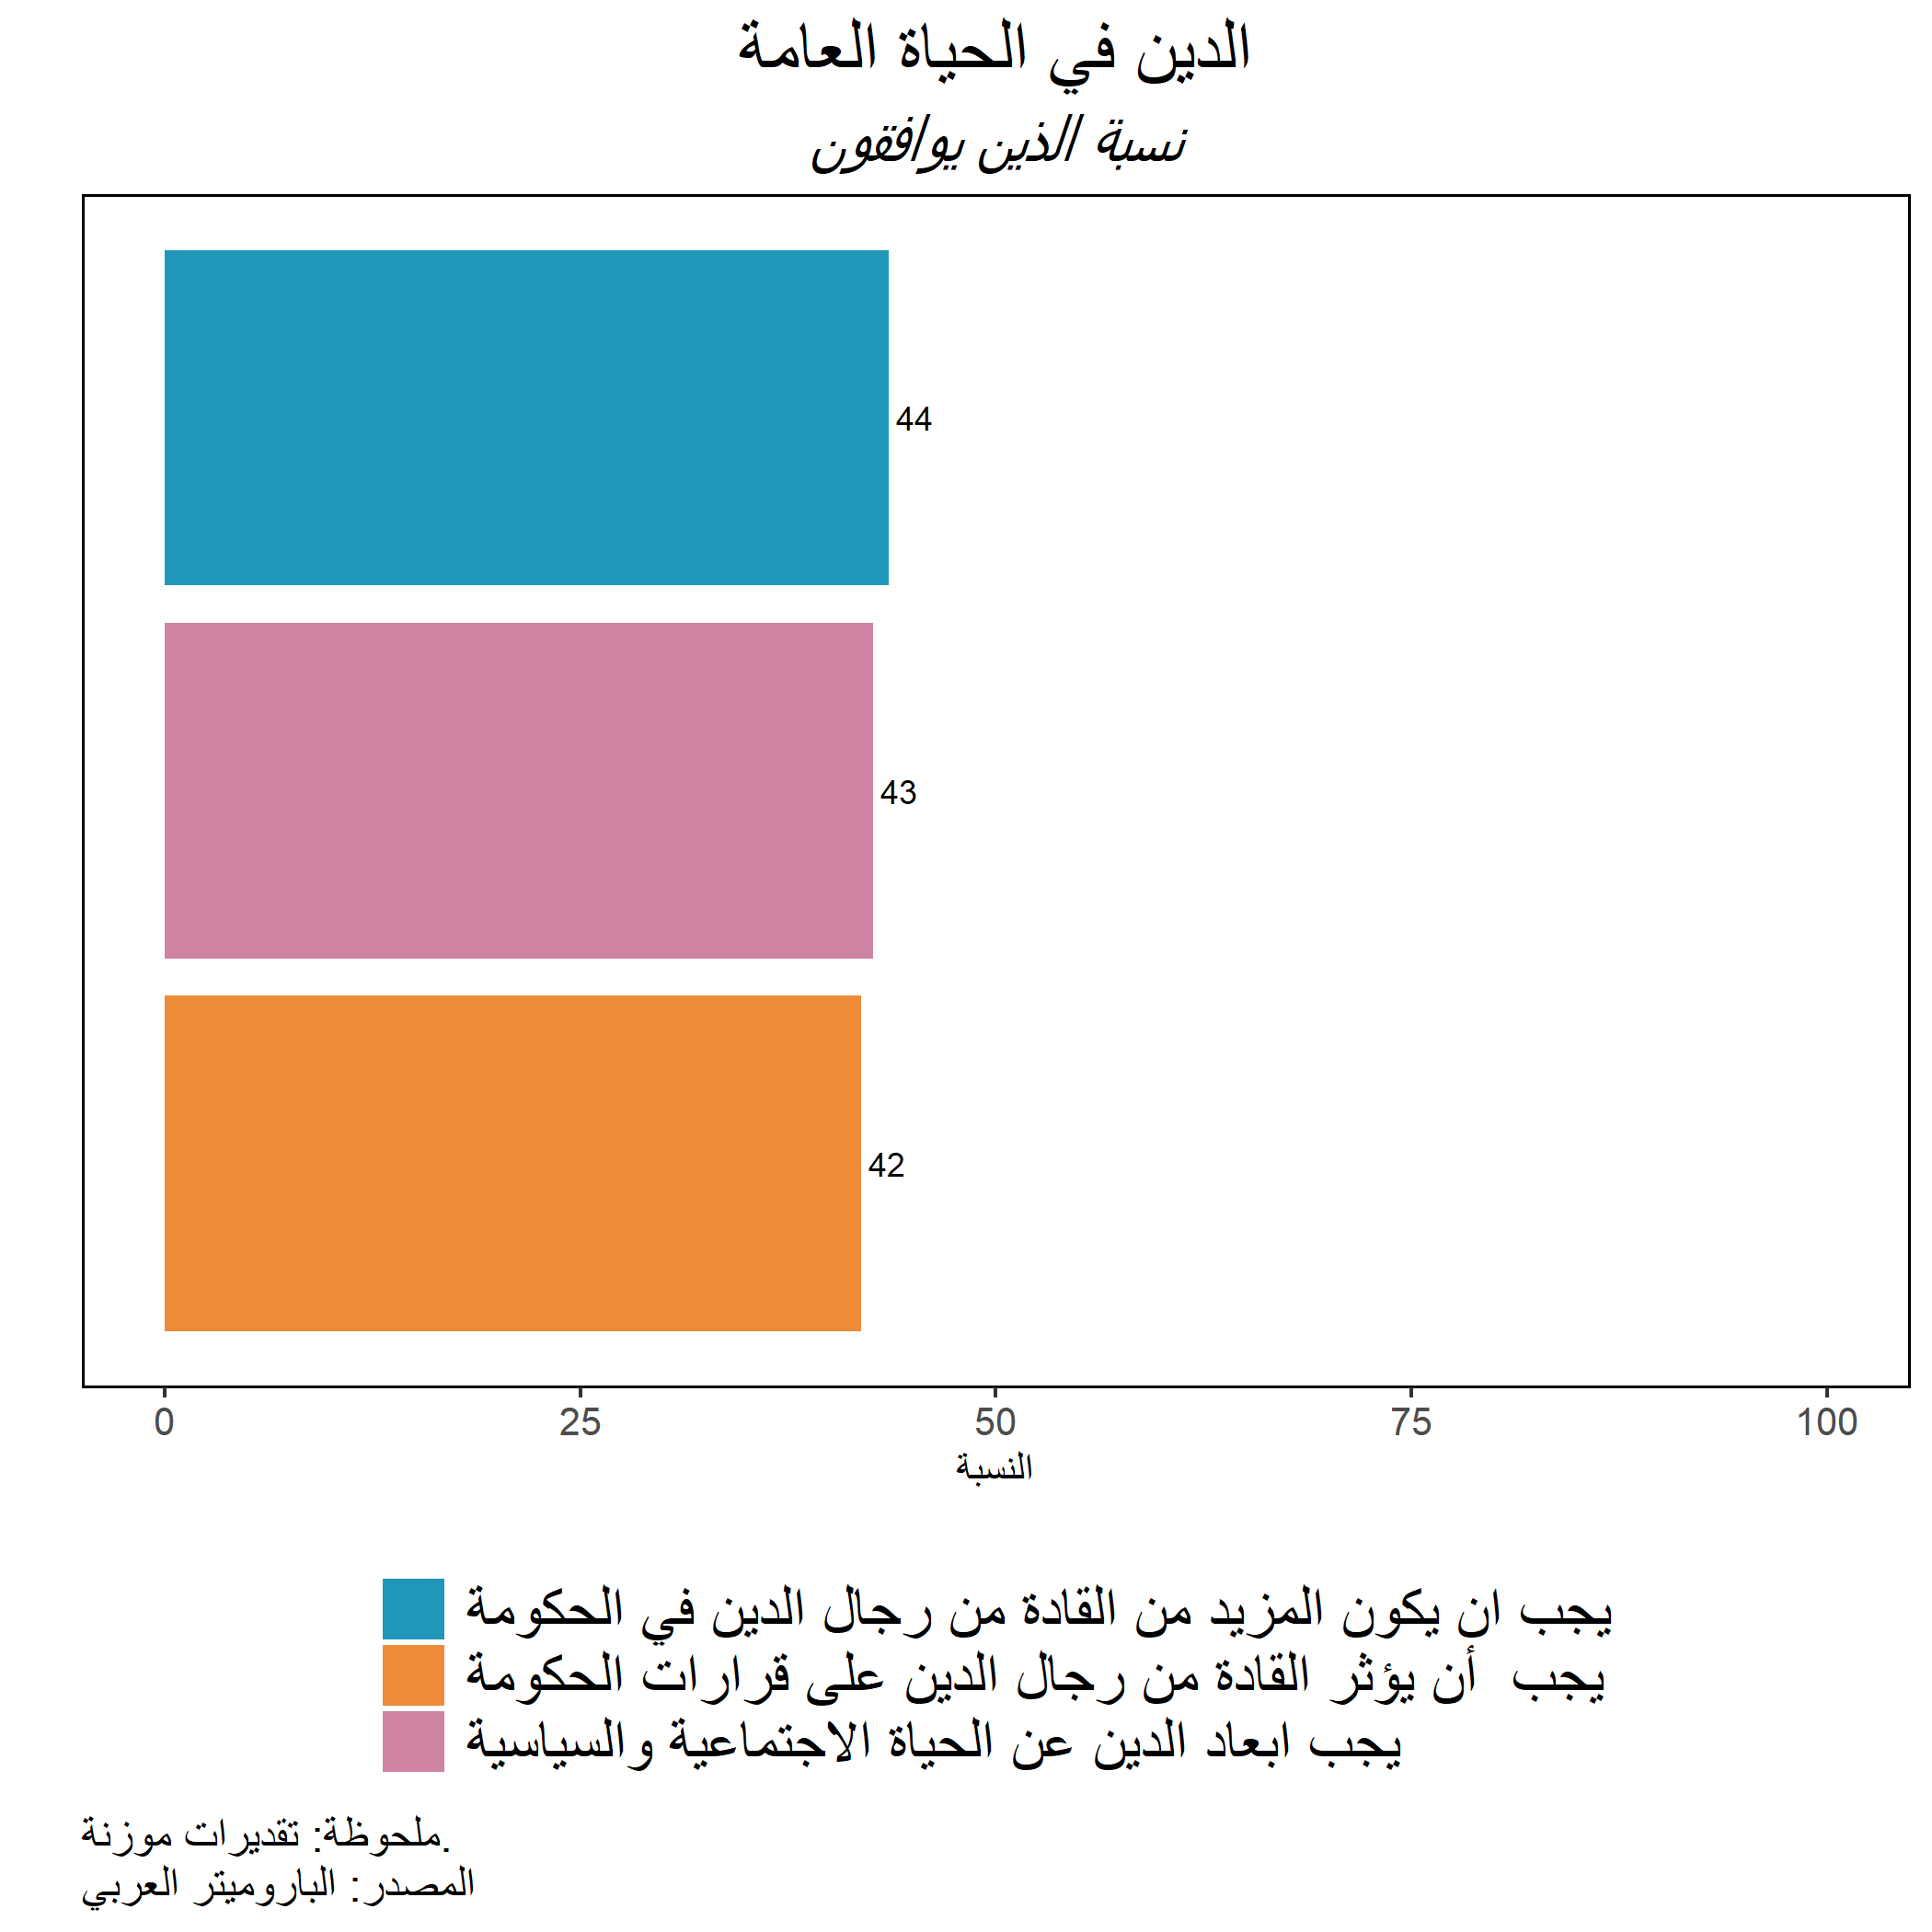
\includegraphics[width=13cm]{Q606.png}
		\end{figure}
	\end{center}
	
 بالمثل، يرى 42 بالمئة ضرورة أن يكون للقادة الدينيين تأثير على قرارات الحكومة، مقارنة بـ 48 بالمئة يخالفون هذه المقولة، وهي النسب التي لم تتغير منذ 2016. وفي الوقت نفسه، لدى طرح سؤال عما إذا كان يجب فصل الدين عن الحياة الاجتماعية والاقتصادية، أيد 43 بالمئة المقولة في حين خالفها 51 بالمئة. من ثم، وانطلاقاً من قياسات متعددة، فإن نصف سكان الجزائر تقريباً مستمرون في الاعتقاد بضرورة وجود دور للدين في الحياة العامة، في حين تعارض هذا الأمر نسبة مماثلة.
	
 وعلى الرغم من أن الاختلاف بسيط في التوجهات بحسب السن والنوع الاجتماعي والدخل والسكن بالحضر أو الريف، فإن أصحاب التعليم الأعلى أقل تفضيلاً لدور الدين في السياسة. وفي الوقت نفسه، فإن سكان الشمال الشرقي هم الأكثر إقبالاً على دعم دور الدين في السياسة، في حين أن سكان الشمال الغربي هم الأقل إقبالاً على هذا الرأي.
	
 ورغم انقسام الجزائريين حول دور الدين في الحياة العامة، فهناك دعم عام لفكرة أن تستند قوانين الجزائر إلى الشريعة. إجمالاً، يقول 43 بالمئة إن قوانين البلاد يجب أن تستند إلى الشريعة بالكامل (15 بالمئة) أو في الأغلب الأعم (28 بالمئة). وفي الوقت نفسه يقول 39 بالمئة إنها يجب أن تستند بنسب متساوية إلى الشريعة وإلى إرادة الشعب، في حين يرى 14 بالمئة فقط أن تستند القوانين بشكل كامل أو في الأغلب على إرادة الشعب.

\section*{العلاقات الدولية}

 مقارنة بدول أخرى في الشرق الأوسط وشمال أفريقيا، فإن قلة من الجزائريين يرغبون في علاقات اقتصادية أقوى أو زيادة الدعم الأجنبي لبلدهم. على سبيل المثال، فإن الربع (24 بالمئة) يرغبون في تقوية العلاقات بالولايات المتحدة الأمريكية، وهي أقل نسبة بين دول الشرق الأوسط وشمال أفريقيا. ولقد انحسرت هذه النسبة بثبات منذ عام 2013، فتراجعت 19 نقطة مئوية على مدار الفترة المذكورة. ويجدر بالملاحظة أن الحاصلين على مستويات تعليمية أفضل ومن يعيشون خارج منطقة العاصمة هم الأكثر تقبلاً بكثير لتقوية العلاقات بالولايات المتحدة الأمريكية.
	
		\begin{center}
		\begin{figure}[H]
			\centering
			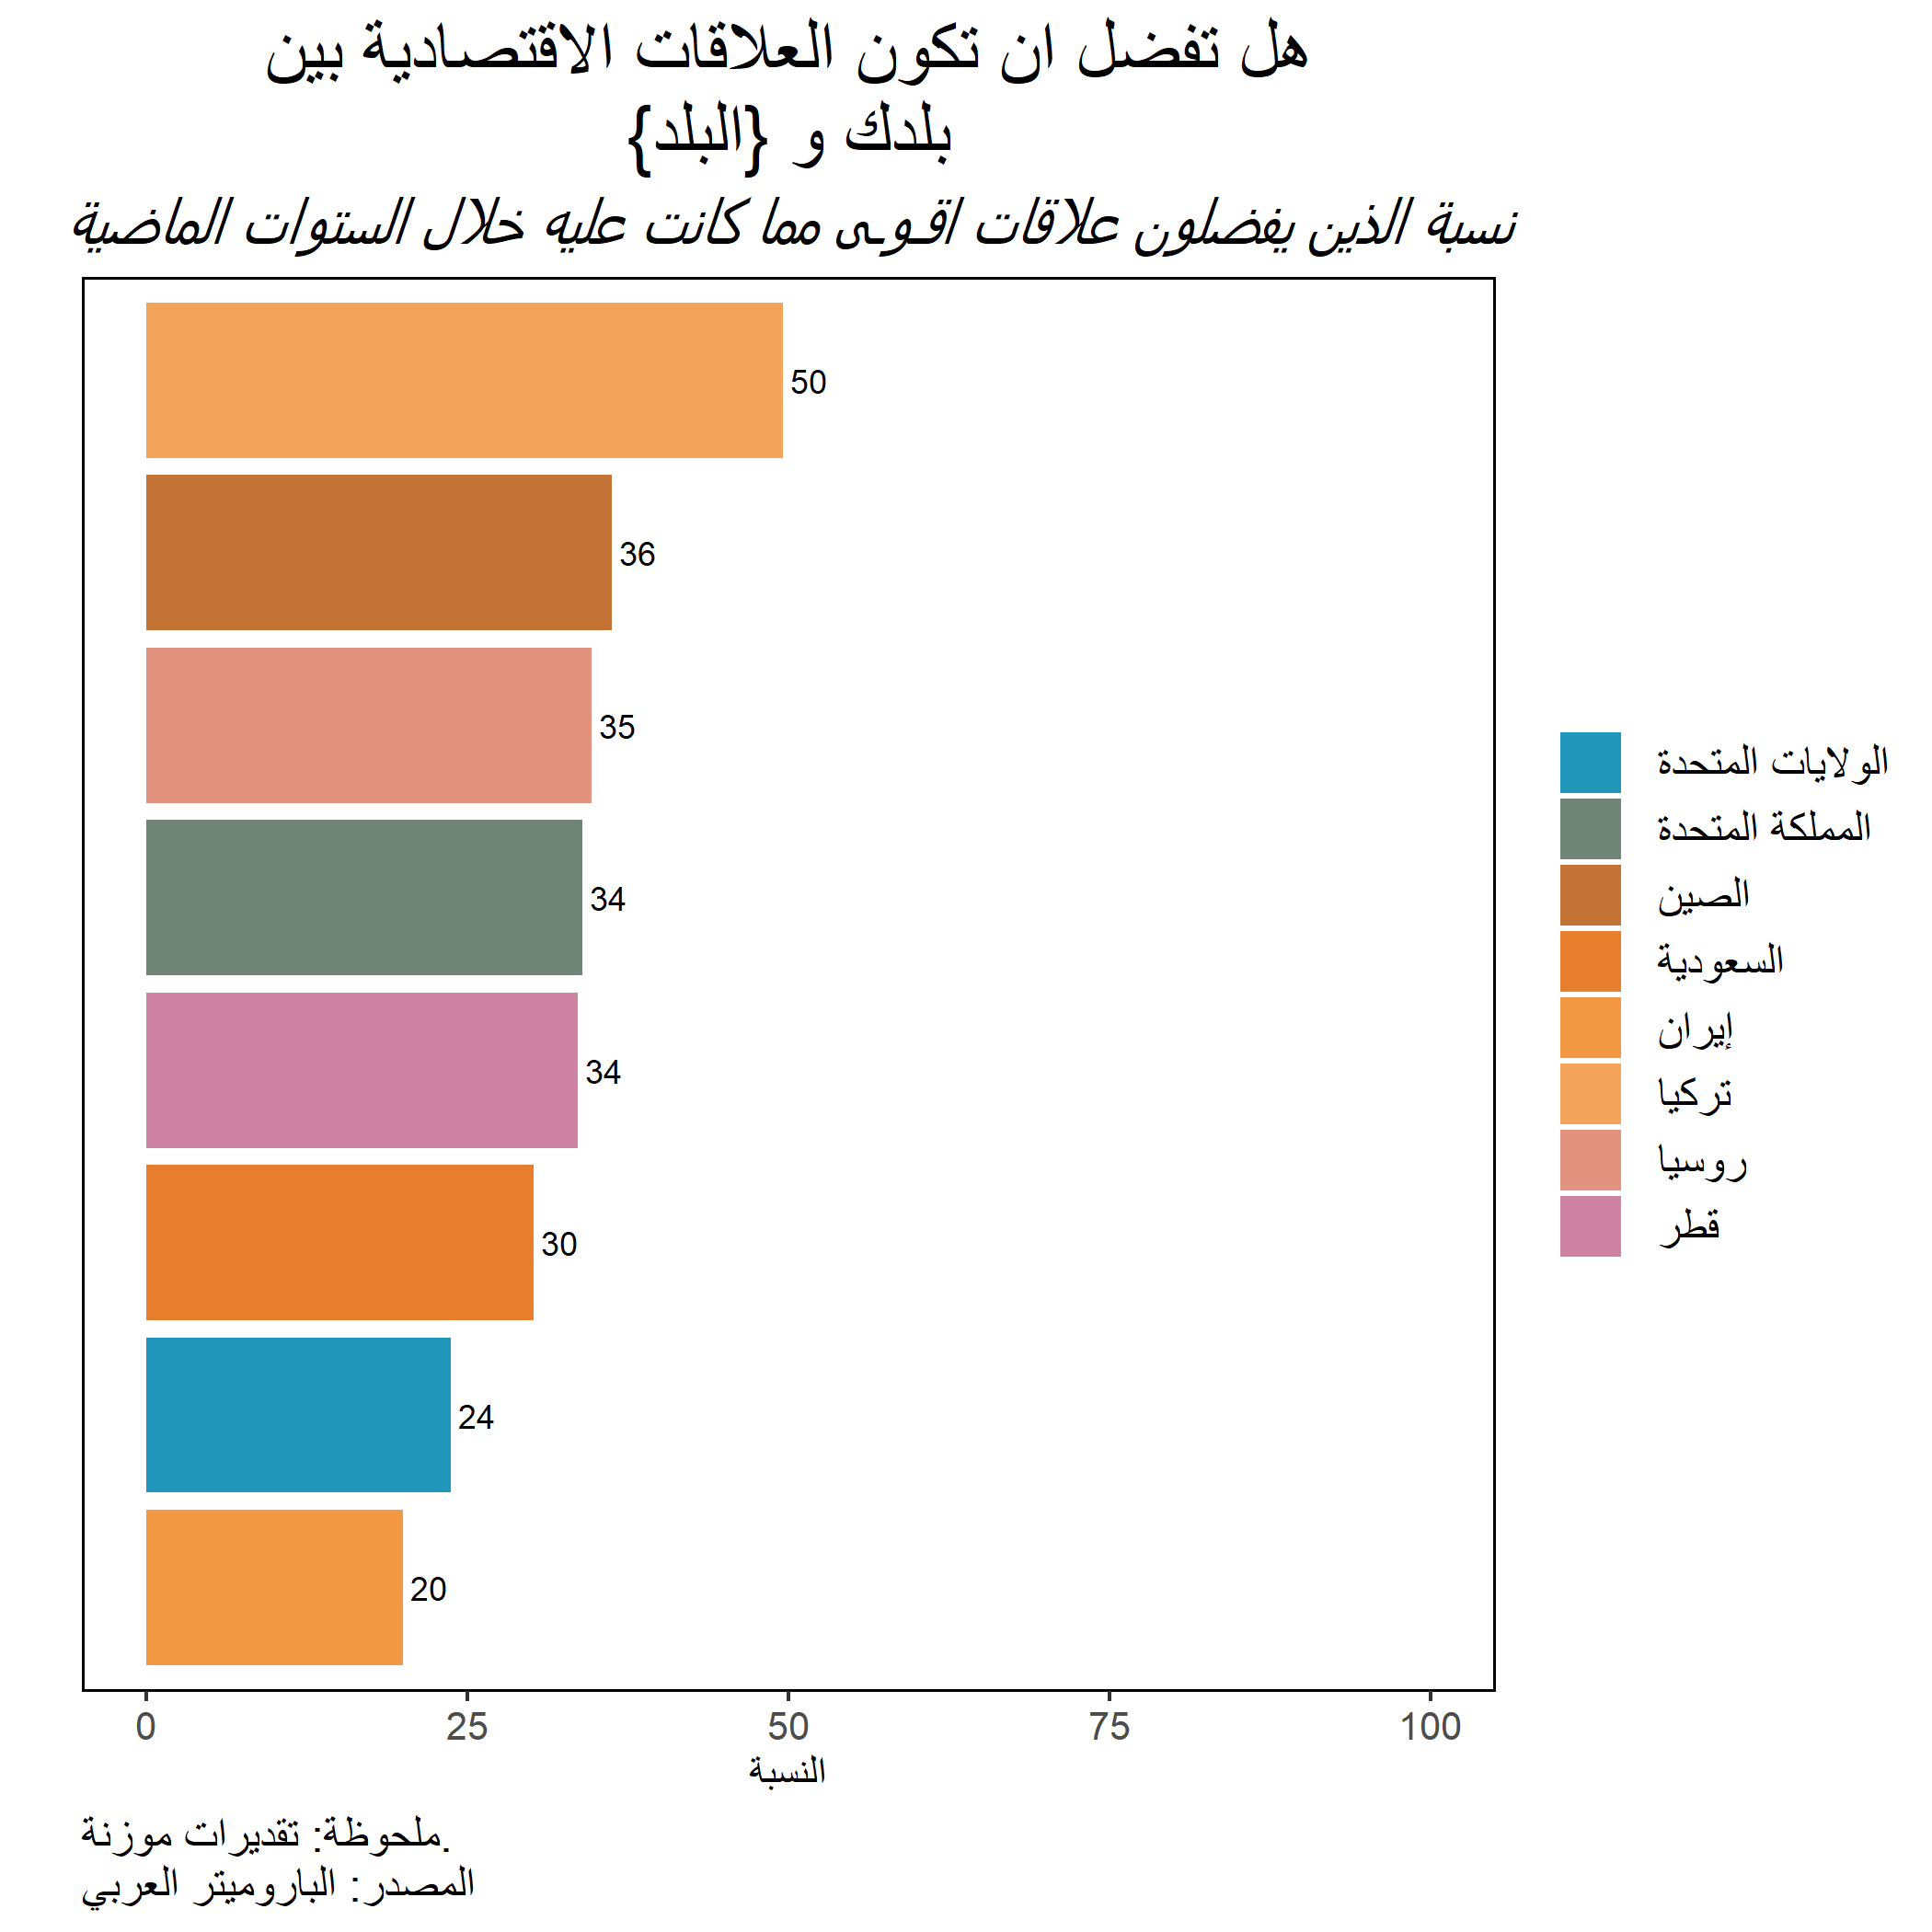
\includegraphics[width=13cm]{Q700.png}
		\end{figure}
	\end{center}
	
 وتعد نسب الإقبال على الرغبة في تقوية العلاقات بالقوى العالمية الأخرى أعلى إلى درجة ما. فعلى سبيل المثال، يفضل الثلث تقريباً تقوية العلاقات بالصين (36 بالمئة) أو روسيا (35 بالمئة). 
	
 ومن بين القوى الإقليمية، يرغب 3 من كل 10 أشخاص فحسب في تقوية العلاقات بالسعودية، وهي النسبة التي تراجعت 18 نقطة مئوية منذ 2013. ونسبة الرغبة في تقوية العلاقات بقطر أعلى قليلاً (34 بالمئة) وإن كانت تركيا هي التي حصدت أعلى درجة دعم من بين القوى الإقليمية، إذ يرغب النصف في تقوية العلاقات بها. وفي الوقت نفسه فإن إيران هي الأقل شعبية، إذ لا يرغب سوى شخص من كل 5 أشخاص في تقوية العلاقات بها.
	
 ومن جانب آخر، فإن دعم زيادة المساعدات الأجنبية محدود. فالربع تقريباً (27 بالمئة) يرغبون في زيادة المساعدات من الولايات المتحدة الأمريكية، مقارنة بـ 32 بالمئة يرغبون في زيادة المساعدات من روسيا، و38 بالمئة في حالة الصين. والرغبة في المساعدات الإضافية من القوى الإقليمية محدودة بدورها. وفي الوقت نفسه فإن الثلث فقط (34 بالمئة) يرغبون في مساعدات إضافية من السعودية. هذا التردد إزاء المساعدات الأجنبية يرجع – جزئياً – على الأرجح إلى أن أكثر من النصف (55 بالمئة) يقولون إن الدافع الرئيسي وراء تقديم الدول الغربية للمساعدات هو كسب النفوذ على بلدهم.
	
 ورغم الإحجام عن الرغبة في تقوية العلاقات الاقتصادية أو زيادة المساعدات الخارجية، فإن الجزائريين يدعمون بشكل متزايد الانفتاح على العالم الخارجي؛ إذ يقول 4 من كل 10 أشخاص إن من الأفضل لبلدهم أن ينفتح بدرجة أكبر، مقارنة بـ 32 بالمئة كانوا يتبنون هذا الرأي في عام 2013.

%%%%%%%%%%%%%%%%%%%%%%%%%%%%%%
%%%%% 
%%%%%%%%%%%%%%%%%%%%%%%%%%%%%%%%%%% 
\newpage
\pagestyle{empty}
\backgroundsetup{
	scale=1,
	color=black,
	opacity=1,
	angle=0,
	contents={%
		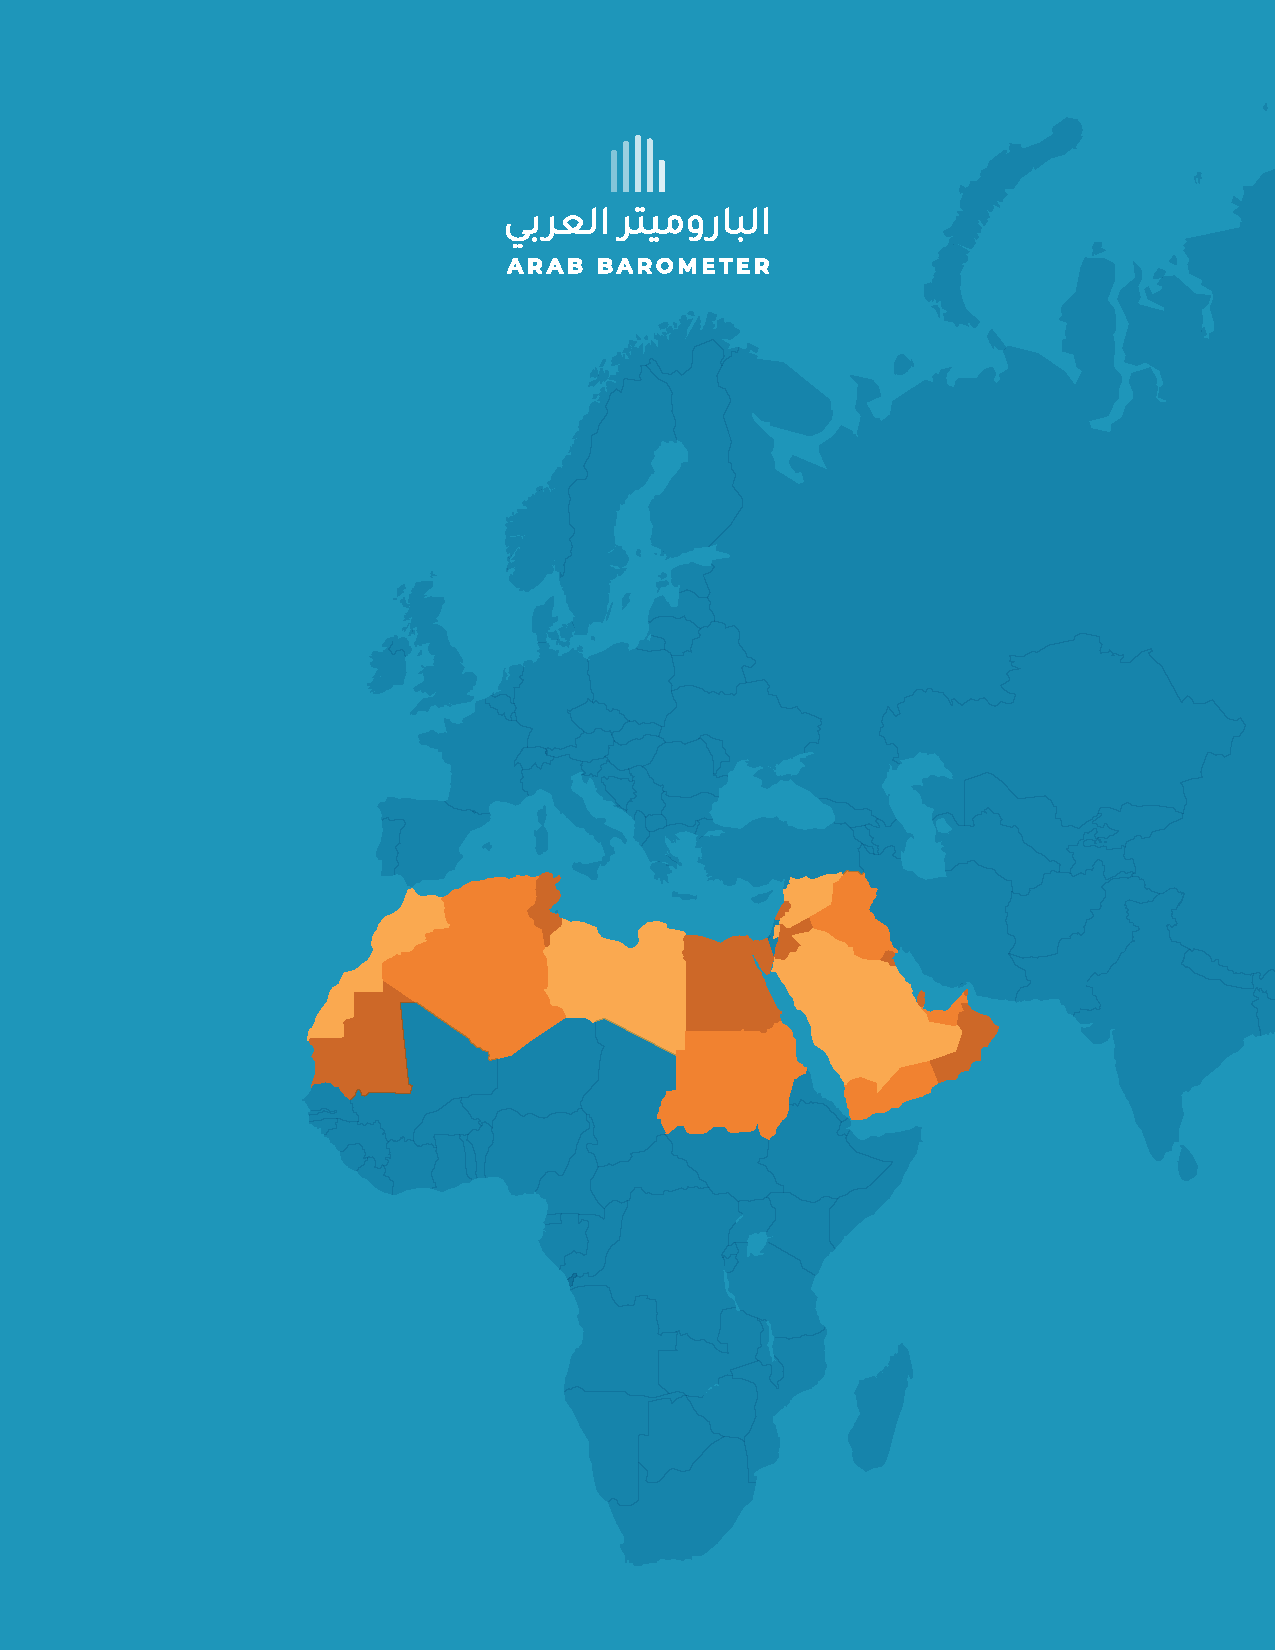
\includegraphics[width=\paperwidth,height=\paperheight]{AB_FrontCover.pdf}
	}%
}
\newgeometry{left=1.5in,right=1.5in,top=1in, bottom=1in}
\pagestyle{empty} 
\vspace*{1in}
\centering
\textbf {\LARGE \color{white} 	\href{http://www.arabbarometer.org/about}{عن الباروميتر العربي}} 
\vspace*{0.2in}
\normalsize \color{white}{الباروميتر العربي هو شبكة بحثية مستقلة وغير حزبيّة، تقدم نظرة ثاقبة عن الإتجاهات والقيم الإجتماعية والسياسية والإقتصادية للمواطنين العاديين في العالم العربي. 
 \\
	\vspace*{0.2in}
تقوم الشبكة بإجراء إستطلاعات للرأي العام في الشرق الأوسط وشمال أفريقيا ذات مستوى عالٍ من الجودة والمصداقية منذ عام 2006 \\
	\vspace*{0.2in}
نحن أضخم مستودع للبيانات المتاحة في متناول العامة حول آراء الرجال والنساء في المنطقة. تمنح نتائج استطلاعاتنا فسحة للمواطنين العرب للتعبير عن احتياجاتهم واهتماماتهم.
 \\	
	\vspace*{4.1in}	
	\begin{tabular}{R {2.2in} R {2in} R {2in}}
		\Huge \color{abblue}{
			\href{http://www.arabbarometer.org}{..........} }&
		\Huge \color{abblueD}{\href{http://www.facebook.com/arabbarometer/}{..........} }&	
		\Huge \color{abblue}{
			\href{https://twitter.com/arabbarometer}{..........}}\\
	\end{tabular}

\end{document}